\chapter{Gaussian processes}\label{gaussianProcessChapter}
This chapter introduces the \textbf{Gaussian processes}. Inevitably, the chapter will not be exhaustive of the subject, but its main features of interest for the purposes of the paper will be treated. For this reason, the discussion will not be devoted to framing Gaussian processes in the vast context of stochastic processes and will limit itself to a focused study of its peculiarities.\\
The python codes used in the chapter require executing the \ref{import} and \ref{import2} import codes of the libraries. Furthermore, the cubic mean is defined for all kernels as in the code \ref{cubedMean}. 
The code for the kernel images is inspired by that written by Peter Roelants in his blog on the page "\href{https://peterroelants.github.io/posts/gaussian-process-tutorial/#Gaussian-processes-(1/3)---From-scratch}{Gaussian processes - From scratch}". Important changes have been made to the code, in particular the kernels implemented by the scikit-learn library are used.
The code for data prediction, on the other hand, takes its inspiration from \href{https://docs.w3cub.com/about/}{W3cubDocs} on the page "\href{https://docs.w3cub.com/scikit_learn/auto_examples/gaussian_process/plot_gpr_noisy_targets}{Gaussian Processes regression: basic introductory example}". Again, important changes have been made in the code.
The code about the concentration of $CO_2$ is a modification of the code '\href{https://scikit-learn.org/stable/auto_examples/gaussian_process/plot_gpr_co2.html}{Gaussian process regression (GPR) on Mauna Loa CO2 data}' present in the scikit-learn documentation.\\
The sources used for the drafting of the chapter are: \cite{rasmussen_gaussian_2006}, \cite{murphy_probabilistic_2022}, \cite{rasmussen_gaussian_2004}, \cite{duvenaud_automatic_2014}, \cite{gortler_visual_2019}, \cite{murphy_machine_2012}.


\begin{textblock*}{0.64\textwidth}(3.5cm+0.36\textwidth,18.5cm)
\epigraph{In applying mathematics to subjects such as physics
or statistics we make tentative assumptions about the
real world which we know are false but which we believe
may be useful nonetheless. The physicist knows that
particles have mass and yet certain results, approximating
what really happens, may be derived from the assuhption that they do not. Equally, the statistician knows, for
example, that in nature there never was a normal distribution, there never was a straight line, yet with normal and
linear assumptions, known to be false, he can often derive
results which match, to a useful approximation, those
found in the real world.}{George E. P. Box}
\end{textblock*}

\newpage


%%%%%%%%%%%%%%%%%%%%%%%%%%%%%%
%%%%% DEFINIZIONE
%%%%%%%%%%%%%%%%%%%%%%%%%%%%%%
\section{Definition and motivation}


\begin{defi}[Gaussian process]
  A \textbf{Gaussian process} is a set of random variables such that every finite subset of it has a multivariate Gaussian distribution.
\end{defi}

It is evident from the definition that the theory of multivariate Gaussian distributions has considerable importance in the study of Gaussian processes.\\
Similar to the Gaussian distribution, which is completely determined by its mean vector and covariance matrix, Gaussian processes are completely determined by a \textit{mean function} (which determines its mean), denoted $m(x)$, and by a \textit{covariance function} (which determines the covariance), denoted $k(x,x')$. The role of the two functions will be discussed in more detail in the next section.\\
Despite this similarity, however, Gaussian distributions and Gaussian processes differ in one important characteristic: the former work with vectors, the latter with functions.

\vspace{0.5cm}

\begin{oss}[Motivation: nonlinear regression]
  The main application of Gaussian processes, and the main theme of this chapter, is \textbf{nonlinear regression}.\\
  While the linear regression model seeks, from observed data, a linear relationship between a dependent variable $Y$ and an independent variable $x$, taking into account a statistical error $\epsilon$, in the form $Y_i=\beta_0+\beta_1 x_i+\epsilon_i$, where the unknowns are $\beta_0$ and $\beta_1$; nonlinear regression is a form of regression in which the function expressing the relationship between independent and dependent variables is a nonlinear combination of the model parameters and depends on one or more independent variables, thus in the form: $Y=f(X,\theta)+\epsilon$, where the unknowns are $\theta$ and the function $f$.\\
  An important difference between the two types of regression is that for nonlinear regression, unlike linear regression, there is no general method for determining parameter values. 

%%%%%%%%%%%%%%%%%%%%%%%%%%%%%%%%%%%
%%%%%% IMMAGINE REGRESSIONE NONLINEARE
%%%%%%%%%%%%%%%%%%%%%%%%%%%%%%%%%%%
\begin{figure}[h]
\centering
\begin{subfigure}{.5\textwidth}
  \centering
  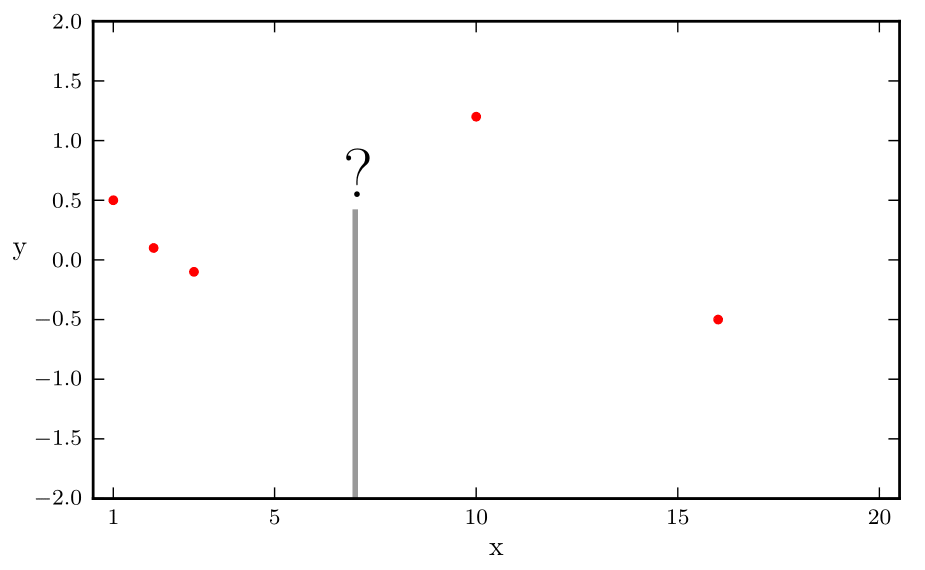
\includegraphics[width=\linewidth]{images/Gaussian process/motivazione2.png}
\end{subfigure}%
\begin{subfigure}{.5\textwidth}
  \centering
  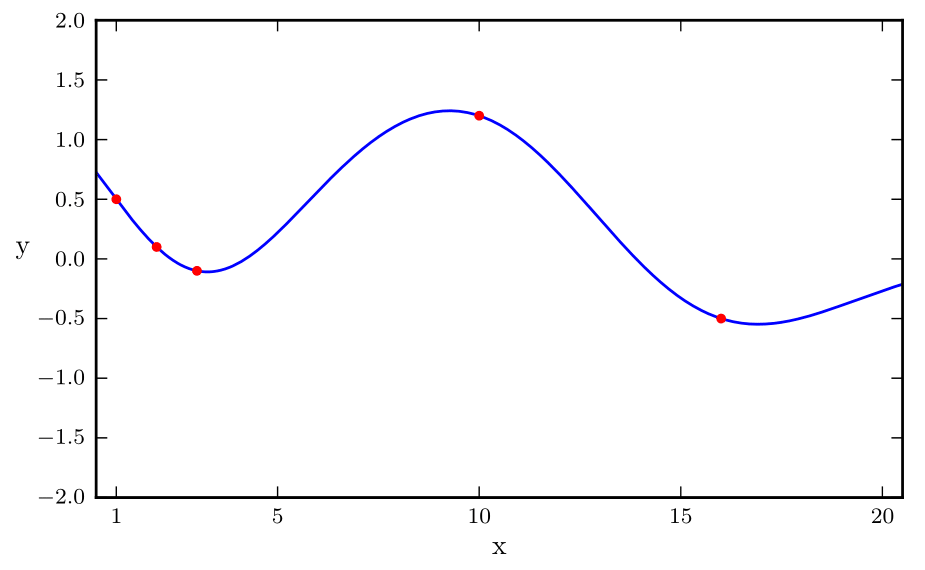
\includegraphics[width=\linewidth]{images/Gaussian process/motivazione3.png}
\end{subfigure}
\caption{Nonlinear regression \cite{turner_gaussian_2016}.}
\end{figure}


\newpage

Gaussian processes provide a good method for the determination of parameters in nonlinear regression not only because they exploit the theory of the multivariate Gaussian distribution, which is overall simple, but because in addition to a function that approximates the data nonlinearly with maximum likelihood (a concept clarified later) they provide an indication of the confidence of the regression in the form of an area within which less likely (but still possible) interpolating functions reside, as illustrated in figure \ref{nonlinearRegressionGaussianProcess}.


%%%%%%%%%%%%%%%%%%%%%%%%%%%%%%%%%%%
%%%%%% IMMAGINE REGRESSIONE NONLINEARE GAUSSIANA
%%%%%%%%%%%%%%%%%%%%%%%%%%%%%%%%%%%
\begin{figure}[h]
    \centering
    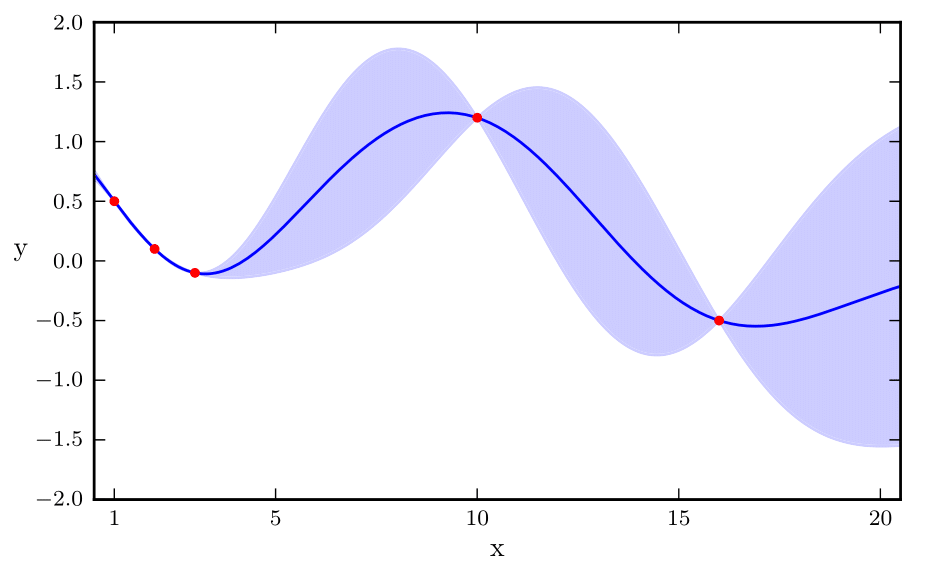
\includegraphics[width=0.85\textwidth]{images/Gaussian process/motivazione4.png}
    \caption{Nonlinear regression with Gaussian processes \cite{turner_gaussian_2016}.}
    \label{nonlinearRegressionGaussianProcess}
\end{figure}

\end{oss}

\newpage

\section{Introduction to Gaussian processes and notation}
Although it is beyond the scope of this paper to go into this in depth, the definition of a stochastic process is given to facilitate the introduction of the notation used.



%%%%%%%%%%%%%%%%%%%%%%%%%%%%
%%%%%% PROCESSO STOCASTICO
%%%%%%%%%%%%%%%%%%%%%%%%%%%%
\begin{defi}[Stochastic process]
  A \textbf{stochastic process} on a probability space $(\Omega, \mathcal{F}, \mathbb{P})$ is a family $\{X_t\}_{t\in T\subset \mathbb{R}}$ of random variables indexed by a parameter $t$.
\end{defi}



It is common to call $t$ the index in order to emphasise the role of time in stochastic processes: a stochastic process generally describes mathematically the temporal evolution of a system characterised by being subject to chance, i.e. a system of which the state at time $t$ cannot be determined with certainty but only by a random variable.\\
In a stochastic system it is therefore only possible to calculate the \textit{probability} that the system is in one of the possible states at time $t>t_0$ if the state at time $t_0$ is known; in a deterministic system, on the other hand, the evolution is described by rules (typically in the form of a differential equation) that allow the state of the system to be precisely determined at each time $t>t_0$ if the state at time $t_0$ is known.




%%%%%%%%%%%%%%%%%%%%%%%%%
%%%%%%% NOTAZIONE
%%%%%%%%%%%%%%%%%%%%%%%%%
\begin{nota}[Functions and indexing in Gaussian processes]
  Writing $f\sim \mathcal{GP}(m,k)$ means that "\textit{ the function $f$ is distributed as a Gaussian process with mean function $m(\cdot)$ and covariance function $k(\cdot,\cdot)$}".\\
  The function thus obtained can be described as:
\[f: \chi \rightarrow \mathbb{R},\]
where $\chi$ is any domain. For each element $x$ in the domain $\chi$ there exists a random variable $f(x)$ with which it is associated.
\end{nota}



\begin{oss}[Versatility of Gaussian processes and generalisation of Gaussian vectors] \label{oss1}
  Note that the domain $\chi$ has no restrictions, a feature that makes Gaussian processes very versatile. Note also that with a finite domain a Gaussian process is a multivariate Gaussian vector. In this sense, as mentioned above, Gaussian processes are a generalisation of multivariate Gaussian vectors. 
\end{oss}


\newpage
%%%%%%%%%%%%%%%%%%%%%
%%%%%% MEAN FUNCTION
%%%%%%%%%%%%%%%%%%%%%
\begin{defi}[Mean function]
Given $f\sim \mathcal{GP}(m,k)$ a Gaussian process, the \textbf{mean function} is a function
\[
m:\chi \rightarrow \mathbb{R}
\]
where $m(x)=\mathbb{E}[f(x)]$.
\end{defi}

\begin{oss}
  For the \textit{mean function} there is no requirement in terms of properties of the function. Typical choices are $m(x)=0$ or $m(x)=c$ with $c$ constant.
\end{oss}

Contrary to \textit{mean function}, the choice of \textit{covariance function} is restricted to a certain class of functions, so some preliminary concepts are introduced before the definition.




%%%%%%%%%%%%%%%%%%%%%%%%
%%%% MERCER KERNEL
%%%%%%%%%%%%%%%%%%%%%%%%
\begin{defi}[Mercer kernel/positive definite kernel]
  A \textbf{Mercer kernel} (or \textbf{positive definite kernel}) is defined as any symmetrical function 
\[
\mathcal{K}: \chi\times\chi \rightarrow \mathbb{R}^+
\]
 such that: $\sum_{i=1}^N\sum_{j=1}^N\mathcal{K}(x_i,x_j)c_ic_j \geq 0$ for any set of distinct elements $\{x_i\}_{i=1}^N\subset \chi$, $\{c_i\}_{i=1}^N\subset  \mathbb{R}$.
\end{defi}

An alternative definition is based on the concept of \textit{Gram matrix}:

\begin{defi}[Gram matrix]
  Given a function $\mathcal{K}: \chi\times \chi\rightarrow \mathbb{R}^+$, let ${x_i}_{i=1}^N\subset \chi$ be any set of distinct elements, we define the \textbf{Gram matrix} of $\mathcal{K}$ to be the following:
\[
\bm{K}=\begin{pmatrix}
    \mathcal{K}(x_1,x_1) & \mathcal{K}(x_1,x_2) & \dots & \mathcal{K}(x_1,x_N)\\
    \mathcal{K}(x_2,x_1) & \mathcal{K}(x_2,x_2) & \dots & \mathcal{K}(x_2,x_N)\\
    \vdots & \vdots & \ddots & \vdots\\
    \mathcal{K}(x_N,x_1) & \mathcal{K}(x_N,x_2) & \dots & \mathcal{K}(x_N,x_N)
    \end{pmatrix}
\]
\end{defi}

\begin{defi}[Mercer kernel/positive definite kernel]
Given a function $
\mathcal{K}: \chi\times\chi \rightarrow \mathbb{R}^+
$, $\mathcal{K}$ is called \textbf{Mercer kernel} if and only if its Gram matrix is positive semidefinite.
\end{defi}

It is now possible to define the covariance function.

\newpage


%%%%%%%%%%%%%%%%%%%%%%%%
%%%% COVARIANCE FUNCTION
%%%%%%%%%%%%%%%%%%%%%%%%
\begin{defi}[Covariance/kernel function]
  Given a Gaussian process $f\sim \mathcal{GP}(m,k)$, the \textbf{covariance function} is a function
\[
k:\chi\times \chi \rightarrow \mathbb{R}
\]
such that $k(\cdot,\cdot)$ is a \textit{Mercer kernel}. The following occurs 
\[k(x,x')=\mathbb{E}[(f(x)-m(x))(f(x')-m(x'))]=\text{Cov}[f(x),f(x')].
\]
\end{defi}

\begin{oss}[Similarity between Gaussian processes and multivariate Gaussian distribution]
  The \textit{mean function} was defined without making any restrictions on the properties of the function, while for the \textit{covariance function} it was required that its Gram matrix be semidefinite positive.\\
  This should come as no surprise: as previously mentioned, Gaussian processes generalise the multivariate Gaussian distribution and as explained in the previous chapter (and emphasised in the remark \ref{ossGaussianaMultivariata}) the latter is defined by two parameters: a mean vector, without any restriction, and a covariance matrix, which must be symmetric and semidefinite positive. There is therefore, in this sense too, similarity between Gaussian processes and multivariate Gaussian distributions.
\end{oss}

\vspace{0.5cm}

%%%%%%%%%%%%%%%%%%%%%%%%%%%%
%%%%%%% ESEMPIO GP
%%%%%%%%%%%%%%%%%%%%%%%%%%%
\begin{ese}[Example of a Gaussian process] \label{esempioProcessoGaussiano}
Consider $f\sim \mathcal{GP}(m,k)$, where:
\[
m(x)=\frac{x^2}{4}\qquad k(x,x')=\text{exp}\left( -\frac{1}{2}(x-x')^2\right).
\]
To understand this example of a Gaussian process, consider the graph of some samples of the function $f$. In order not to work in the infinite case, we consider a finite domain.\footnote{Keep in mind that from a theoretical point of view, the Gaussian processes that are considered in this paper are constructed on an infinite domain of real numbers; however, when generating the graphs, one is forced to consider a finite set of points that are then joined to generate the curve. With this (forced) philosophy, the graphs in the next section are constructed.\label{footnote 1}}: $\chi = \left\{x_i \right\}_{i=1}^{n}$. Since $\chi$ is finite, what is obtained by evaluating $m(\cdot)$ and $k(\cdot,\cdot)$ on the domain are a vector $\bm{\mu}$ and a matrix $\bm{\Sigma}$ where:
\[
\begin{split}
\mu_i&=m(x_i)=\frac{x_i^2}{4} \qquad\qquad\qquad\qquad\qquad\qquad i=1,\dots, n \\
\Sigma_{ij}&=k(x_i,x_j)=\text{exp}\left( -\frac{1}{2}(x_i-x_j)^2\right)\qquad i,j=1,\dots, n
\end{split}
\]
It is thus obtained, as anticipated in the remark \ref{oss1}, that for each $x_i$ in the domain $\chi$ the random variable $f(x_i)$ is a Gaussian random variable of mean $\mu_i$ and variance $\Sigma_{ii}$; calling $\bm{f}=(f(x_1), \dots, f(x_n))^{\text{T}}$ we get, i.e: 
\[
\bm{f}\sim \mathcal{N}(\bm{\mu}, \bm{\Sigma}).
\]

\newpage

Having obtained a multivariate $n$-dimensional Gaussian vector, it is natural to use the same method as introduced in the \ref{sezioneCorrelazione} to derive the graph of the "function" (it is actually a vector) $\bm{f}$. The figure \ref{esempioProcessoGaussianoImmagine} shows the "graphs" of four different samples of a Gaussian vector of dimension $n=60$. Note that the shape of the four graphs is quite different from that of figure \ref{correlazione6} as a consequence of the fact that the distributions have different covariance matrixes. This emphasises how important the covariance function is in Gaussian processes, being responsible for the covariance matrix. This topic will be analysed in detail later.\newline
This example clarified what is meant when it is said that Gaussian processes generalise the multivariate Gaussian distribution.

%%%%%%%%%%%%%%%%%%%%%%%%%
%%%%%%%%% IMMAGINE
%%%%%%%%%%%%%%%%%%%%%%%%
\begin{figure}[h]
    \centering
    \includegraphics[width=0.85\textwidth]{images/Gaussian process/esempioProcessoGaussiano.pdf}
    \caption{Four vectors generated by a Gaussian process defined as in the example \ref{esempioProcessoGaussiano}. Code \ref{Example}.}
    \label{esempioProcessoGaussianoImmagine}
\end{figure}

Note that the code \ref{Example} will not generate the same graph as the figure \ref{esempioProcessoGaussianoImmagine} as there is a random component! The same applies to the other codes mentioned in this chapter.
\end{ese}


\newpage


%%%%%%%%%%%%%%%%%%%%%%%%%%
%%%%% SULLE COVARIANCE FUNCTION
%%%%%%%%%%%%%%%%%%%%%%%%%%


\section{On covariance functions}
For a Gaussian process, the covariance function is of fundamental importance: it is in fact the function $k(\cdot,\cdot)$ that determines how the Gaussian process interprets the data: From the definition of the covariance function, various models can be derived, e.g. linear regression \footnote{Please see \cite{rasmussen_gaussian_2006} and \cite{williams_prediction_1998}} or splines \footnote{Please see \cite{kimeldorf_correspondence_1970}}.\\
\begin{oss}[Importance of covariance]
  In the previous chapter, a visual interpretation of the Pearson correlation index was shown in the \ref{sezioneCorrelazione}, and it was clarified how covariance affects the correlation of two random variables.\\
  Thus, the importance of the covariance function in the correlation between the random variables $f(x)$ and $f(x')$ for each $x,x'\in \chi$ is evident. This is why it is significant, when choosing the covariance function, to take into account how it depends on the pair $(x,x')$.
\end{oss}

Following are the three main types of covariance functions according to their dependence on $(x,x')$ where $x,x'\in \mathbb{R}^D$.




%%%%%%%%%%%%%%%%%%%%%%%%%%
%%%%%%% PROPRIETA KERNEL
%%%%%%%%%%%%%%%%%%%%%%%%%%
\begin{defi}[Stationary covariance function]
  A \textbf{stationary} covariance function is a covariance function that depends on $x-x'$.\\
  A covariance function of this type is translation invariant.
\end{defi}

\begin{defi}[Isotropic covariance function]
  A \textbf{isotropic} covariance function is a covariance function that depends on $|x-x'||$.\\
  Such a covariance function is invariant for rigid motions.
\end{defi}

\begin{defi}[Dot product covariance function]
  A \textbf{dot product} covariance function is a covariance function that depends on $x$ and $x'$ only via $x\cdot x'$.\\
  Such a covariance function is invariant for rotations centred in the origin but not for translations.
\end{defi}

The main covariance functions are shown below. As previously mentioned, this can only be an introduction to the possible choices: important aspects of covariance functions concern their generalisation given by the use of the Mahalanobis distance, a correct choice of kernel for numerical optimisation, relation between kernel choice and deep learning for Gaussian processes \footnote{To further elaborate see \cite{murphy_probabilistic_2022}}, adaptation of kernels to multi-dimensional models \footnote{To further elaborate see \cite{duvenaud_automatic_2014}}...\\
With regard to covariance functions, it is in the interests of this paper to understand how these influence the Gaussian process. Together with the following examples, graphs will therefore be given to support this interest.

\newpage

\subsection{Linear kernel}
%%%%%%%%%%%%%%%%%%%%%%%%%
%%%% LINEAR
%%%%%%%%%%%%%%%%%%%%%%%
\begin{defi}[Linear kernel]
  The \textbf{linear kernel} has the form \[
k(x,x')=\sigma_b^2+\sigma_v^2 (x-c)(x'-c).
\]
\end{defi}

The graph of the function $k(x,x')$ is plotted. A straight line with the usual parameters is obtained.
%%%%%%%%%%%%%%%%%%%%%%%%%
%%%%%%%%% IMMAGINE
%%%%%%%%%%%%%%%%%%%%%%%%
\begin{figure}[h]
    \centering
    \includegraphics[width=0.6\textwidth]{images/Gaussian process/Linear Kernel.pdf}
    \caption{Graph of $k(x,x')$ linear kernel, $\sigma_b^2=1$, $\sigma_v^2=1$, $c=-1$ and $x'=1$. Code \ref{linear kernel code}}
    \label{linear kernel}
\end{figure}

\newpage

Figure \ref{10 sample linear kernel zero mean} shows graphs of functions with distribution $f\sim \mathcal{GP}(m,k)$ where $m(x)=0$ and $k(x,x')$ is the linear kernel, $\sigma_b^2=0$, $\sigma_v^2=1$, $c=0$.



%%%%%%%%%%%%%%%%%%%%%%%%%%%%
%%%%%%%% IMMAGINE
%%%%%%%%%%%%%%%%%%%%%%%%%%%
\begin{figure}[h]
    \centering
    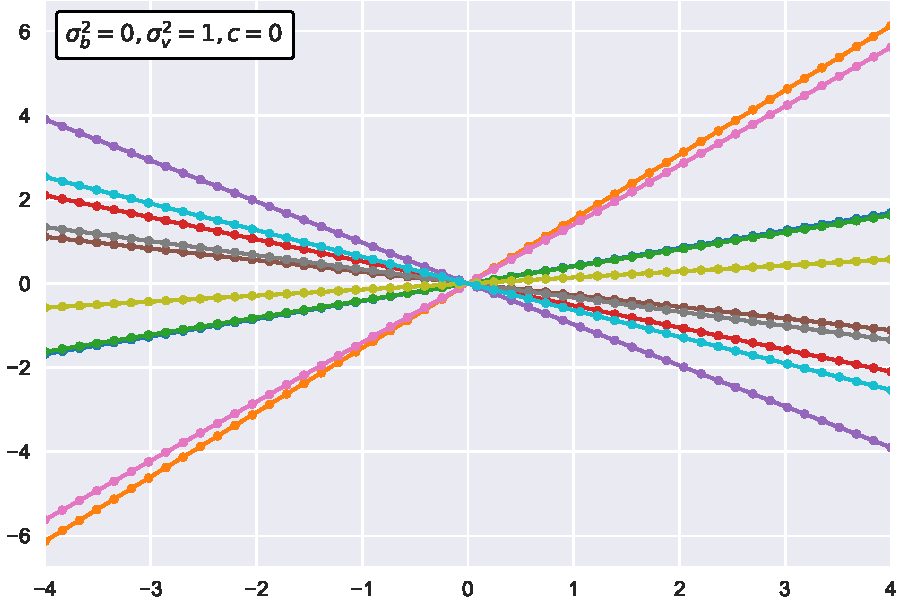
\includegraphics[width=0.85\textwidth]{images/Gaussian process/Linear sample.pdf}
    \caption{Graph of functions with distribution  $f\sim \mathcal{GP}(\bm{0},k)$ where $k(x,x')$ is the linear kernel and $\sigma_b^2=0$, $\sigma_v^2=1$, $c=0$. Code \ref{linear sample}.}
    \label{10 sample linear kernel zero mean}
\end{figure}

Note that the linear kernel generates lines, hence the name.\\
Imposing the mean function equal to zero increases the tendency of lines to pass through the origin. Imposing $m(x)=\alpha\in\mathbb{R}$ increases the tendency of lines to pass through the point $(0,\alpha)$. 
%Esploreremo di seguito l'influenza degli altri parametri del kernel sui grafici delle funzioni, ma è già in parte evidente l'importanza della struttura del kernel nel grafico delle funzioni con distribuzione $\mathcal{GP}(m,k)$.



\newpage






\vspace{1cm}
To understand the influence of parameter $c$, graphs of functions with distribution $f\sim \mathcal{GP}(m,k)$ are shown where $m(x)=0$ and $k(x,x')$ is the linear kernel and the value of $c$ is varied.

%%%%%%%%%%%%%%%%%%%%%%%%%%%%%%%%%%%
%%%%%% IMMAGINI: PARAMETRO c
%%%%%%%%%%%%%%%%%%%%%%%%%%%%%%%%%%%
\begin{figure}[h]
\centering
\begin{subfigure}{.5\textwidth}
  \centering
  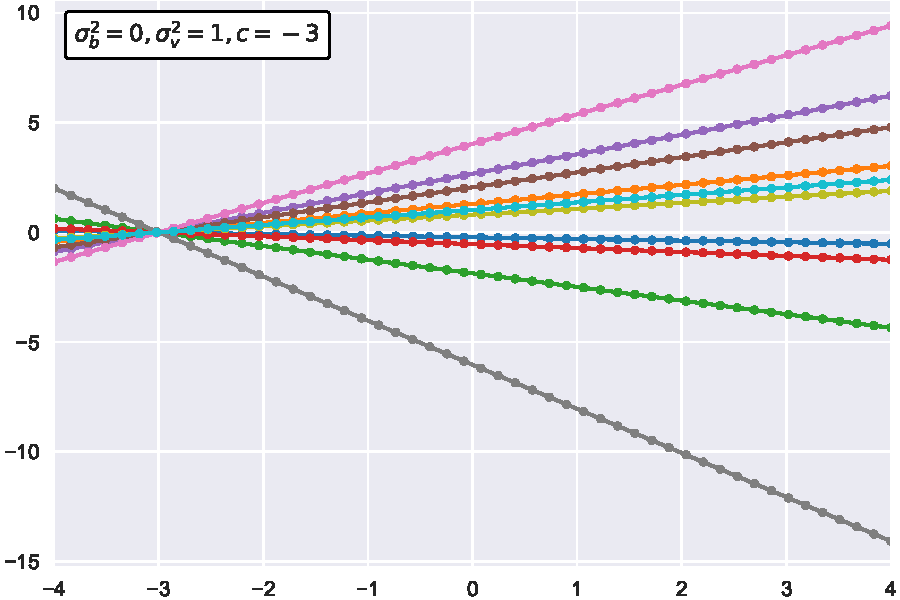
\includegraphics[width=\linewidth]{images/Gaussian process/Linear - c=-3.pdf}
  \caption{$c=-3$}
\end{subfigure}%
\begin{subfigure}{.5\textwidth}
  \centering
  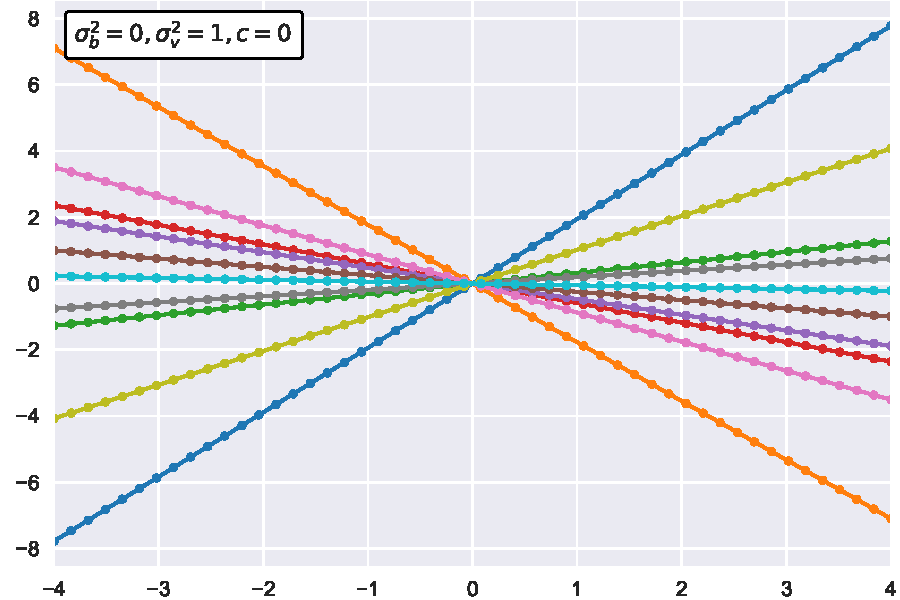
\includegraphics[width=\linewidth]{images/Gaussian process/Linear - c=0.pdf}
  \caption{$c=0$}
\end{subfigure}
\caption{Graph of functions with distribution $f\sim \mathcal{GP}(\bm{0},k)$ where $k(x,x')$ is the linear kernel and $\sigma_b^2=0$, $\sigma_v^2=1$, parameter $c$ is varied. Code \ref{Linear - c}.}
\label{10 sample linear modified c}
\end{figure}


The parameter $c$ therefore imposes a crossing point for all straight lines. Thus $c$ plays the same role as the mean function $m(\cdot)$.

To understand the influence of the parameter $\sigma_b^2$, graphs of functions with distribution $f\sim \mathcal{GP}(m,k)$ are shown where $m(x)=0$ and $k(x,x')$ is the linear kernel and the value of $\sigma_b^2$ is varied.

%%%%%%%%%%%%%%%%%%%%%%%%%%%%%%%%%%%
%%%%%% IMMAGINI: PARAMETRO sigma_b
%%%%%%%%%%%%%%%%%%%%%%%%%%%%%%%%%%%
\begin{figure}[h]
\centering
\begin{subfigure}{.5\textwidth}
  \centering
  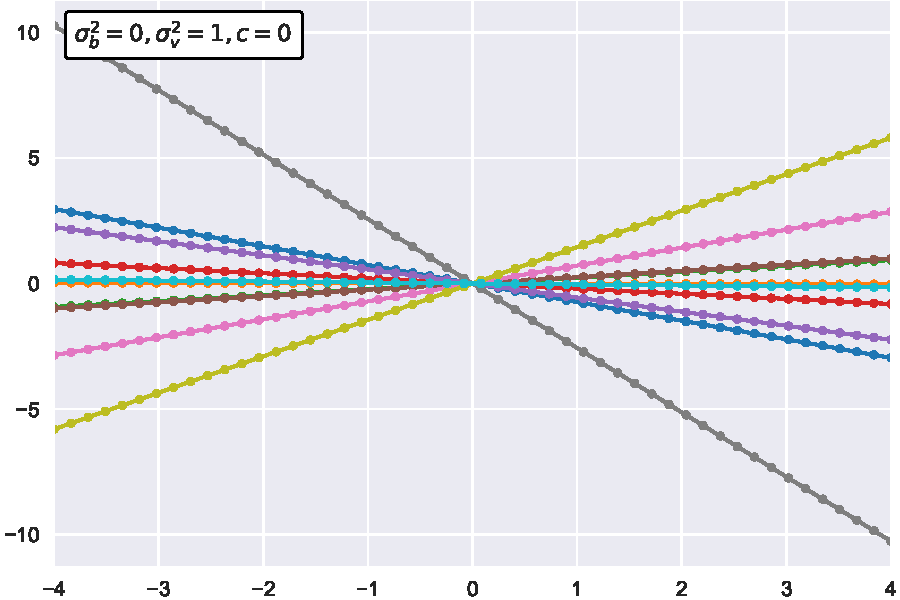
\includegraphics[width=\linewidth]{images/Gaussian process/Linear - sigmab=0.pdf}
  \caption{$\sigma_b^2=0$}
\end{subfigure}%
\begin{subfigure}{.5\textwidth}
  \centering
  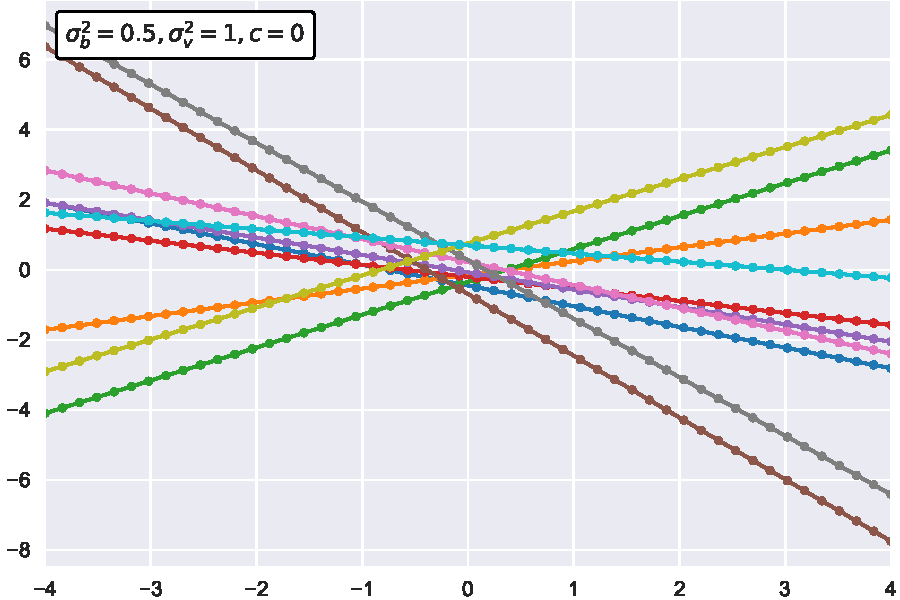
\includegraphics[width=\linewidth]{images/Gaussian process/Linear - sigmab=05.pdf}
  \caption{$\sigma_b^2=0.5$}
\end{subfigure}
\caption{Graph of functions with distribution $f\sim \mathcal{GP}(\bm{0},k)$ where $k(x,x')$ is the linear kernel and $\sigma_v^2=1$, $c=0$, parameter $\sigma_b^2$ is varied. Code \ref{Linear - sigmab}.}
\label{10 sample linear modified sigmab}
\end{figure}
Thus, the parameter $\sigma_b$ influences the precision with which the functions tend to pass through the point $(0,c)$.

\newpage

To understand the influence of the parameter $\sigma_v^2$, graphs of functions with distribution $f\sim \mathcal{GP}(m,k)$ are shown where $m(x)=0$ and $k(x,x')$ is the linear kernel and the value of $\sigma_v^2$ is varied.


%%%%%%%%%%%%%%%%%%%%%%%%%%%%%%%%%%%
%%%%%% IMMAGINI: PARAMETRO sigma_v
%%%%%%%%%%%%%%%%%%%%%%%%%%%%%%%%%%%
\begin{figure}[h]
\centering
\begin{subfigure}{.5\textwidth}
  \centering
  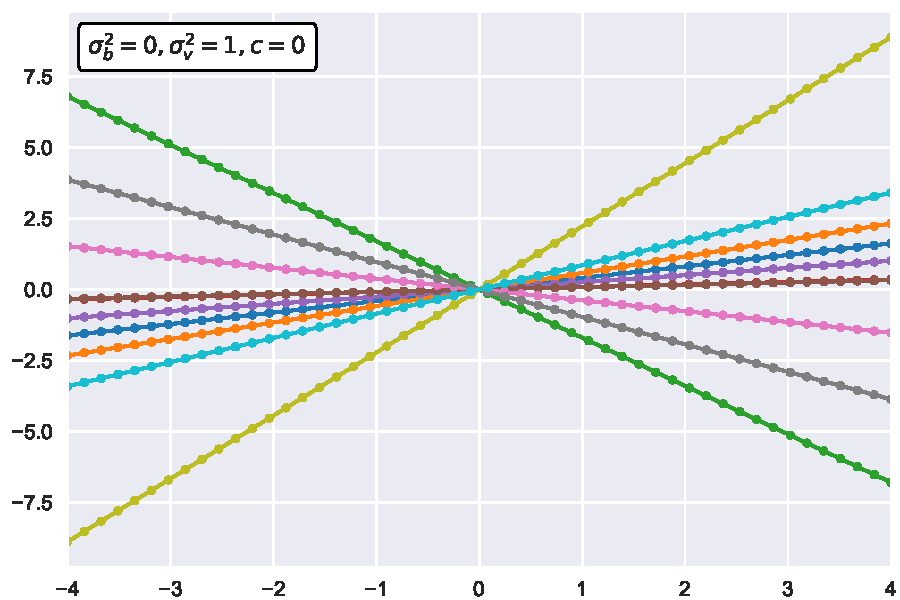
\includegraphics[width=\linewidth]{images/Gaussian process/Linear - sigmav=1.pdf}
  \caption{$\sigma_v^2=1$}
\end{subfigure}%
\begin{subfigure}{.5\textwidth}
  \centering
  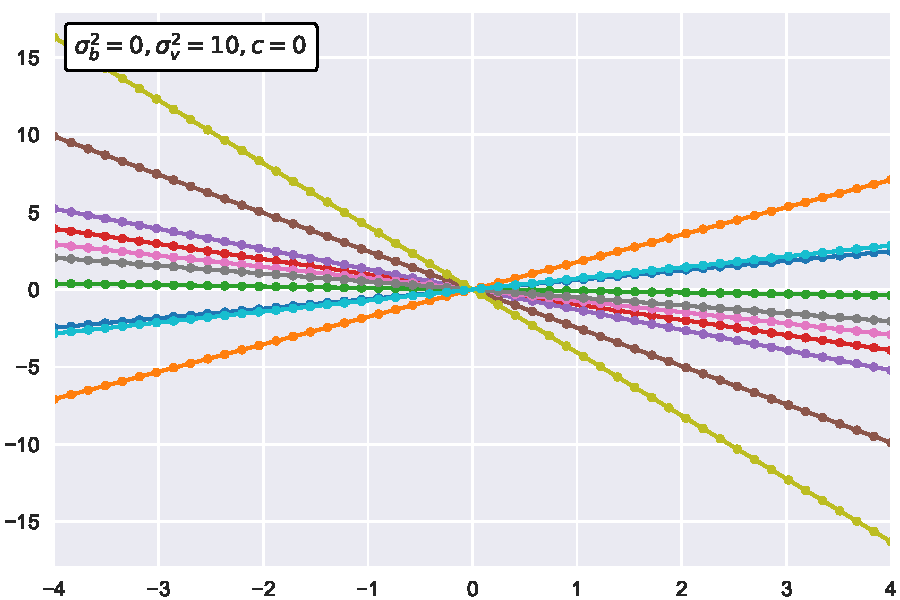
\includegraphics[width=\linewidth]{images/Gaussian process/Linear - sigmav=10.pdf}
  \caption{$\sigma_v^2=10$}
\end{subfigure}
\caption{Graph of functions with distribution $f\sim \mathcal{GP}(\bm{0},k)$ where $k(x,x')$ is the linear kernel and $\sigma_b^2=0$, $c=0$, parameter $\sigma_v^2$ is varied. Code \ref{Linear - sigmav}.}
\label{10 sample linear modified sigmav}
\end{figure}

So the parameter $\sigma_v^2$ influences the slope of the lines, which is proportional to its value.

To understand the influence of the mean function, graphs of functions with distribution $f\sim \mathcal{GP}(m,k)$ where $m(x)=x^3$ and $k(\cdot,\cdot)$ is the linear kernel are shown below.


%%%%%%%%%%%%%%%%%%%%%%%%%%%%
%%%%%%%% IMMAGINE
%%%%%%%%%%%%%%%%%%%%%%%%%%%
\begin{figure}[h]
    \centering
    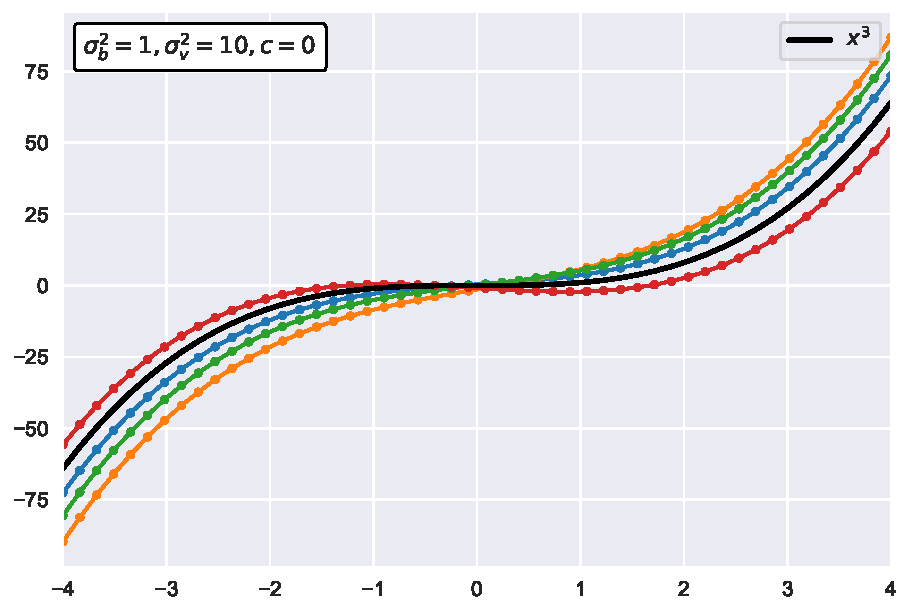
\includegraphics[width=0.85\textwidth]{images/Gaussian process/Linear - cubedmean.pdf}
    \caption{Graph of functions with distribution $f\sim \mathcal{GP}(m,k)$ where $m(x)=x^3$ e $k(x,x')$ is the linear kernel, $\sigma_b^2=1$, $\sigma_v^2=10$, $c=0$. Code \ref{linear cubedmean}.}
    \label{10 sample linear kernel cubed mean}
\end{figure}


\newpage

It is evident from the graph that the graphs resemble the function $x^3$. It will become clearer in the next kernel examples, but from the definition of a Gaussian process (thinking of the multivariate Gaussian distribution, which generalises) every point can be interpreted as a sample of a Gaussian distribution. Recalling the observation \ref{normal decomposition}, we know that every normal (univariate) distribution is decomposable into $Y=\mu+\sigma Z$ where $Z\sim \mathcal{N}(0,1)$; therefore every point $x_i$ on the graph of a function with distribution the Gaussian process as in figure \ref{10 sample linear kernel cubed mean} has decomposition $x_i^3+k(x_i,x_i)Z$. It is therefore clear from the decomposition of each point that the graphs will add to the function $x^3$ an addend due to the covariance function.





\subsection{Squared-exponential kernel}
%%%%%%%%%%%%%%%%
%%% SQUARED-EXPONENTIAL
%%%%%%%%%%%%%


%% A volte è usata ||x-x'||
\begin{defi}[Squared-exponential kernel]
  The \textbf{squared-exponential kernel} has form:
\[
k(x,x')=\sigma^2 \text{exp}\left( -\frac{(x-x')^2}{2l^2} \right).
\]
It is therefore an isotropic covariance function.
\end{defi}

The graph of the function $k(x,x')$ is shown. Note that the parameter $\sigma^2$ affects the peak of the function, while the parameter $l$ affects it indirectly by modifying the rate at which it cancels.



%%%%%%%%%%%%%%%%%%%%%%%%%
%%%%%%%%% IMMAGINE
%%%%%%%%%%%%%%%%%%%%%%%%
\begin{figure}[h]
    \centering
    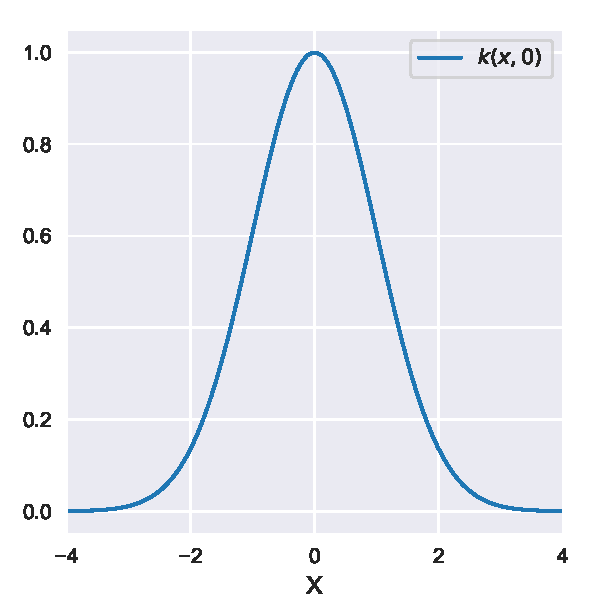
\includegraphics[width=0.6\textwidth]{images/Gaussian process/Squared-exponential kernel.pdf}
    \caption{Graph of $k(x,x')$ squared-exponential kernel, $\sigma^2=1$ and $l^2=1$. Code \ref{squared-exponential}.}
    \label{squared-exponential kernel}
\end{figure}

\newpage

Una funzione distribuita come il processo gaussiano con questo tipo di kernel è $C^\infty$. Esistono diverse variazioni di questo kernel codificanti ipotesi leggermente diverse
A distributed function such as the Gaussian process with this type of kernel is $C^\infty$. There are several variations of this kernel encoding slightly different assumptions about the continuity (even local) of the function, but these are not in the interest of the paper. \footnote{For more details see \cite{duvenaud_automatic_2014}}
\vspace{0.5cm}\\

Shown below are graphs of functions with distribution $f\sim \mathcal{GP}(m,k)$ where $m(x)=0$ and $k(x,x')$ is the squared-exponential kernel.


%%%%%%%%%%%%%%%%%%%%%%%%%
%%%%%%%%% IMMAGINE
%%%%%%%%%%%%%%%%%%%%%%%%
\begin{figure}[h]
    \centering
    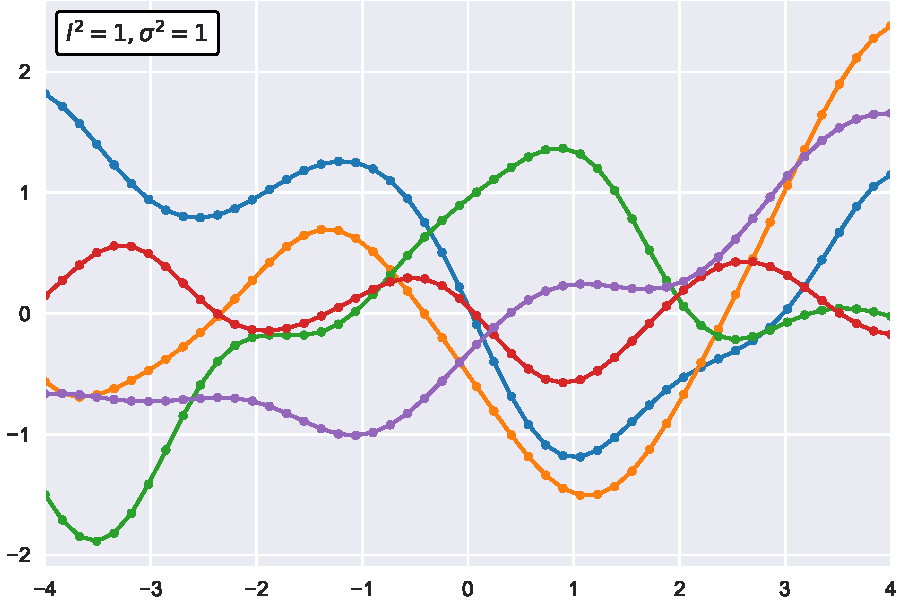
\includegraphics[width=0.85\textwidth]{images/Gaussian process/RBFSample.pdf}
    \caption{Graph of functions with distribution $f\sim \mathcal{GP}(\bm{0},k)$ where $k(x,x')$ is the squared-exponential kernel and $l^2=1$, $\sigma^2=1$. Code \ref{RBF sample}.}
    \label{10 sample exponential kerne zero mean}
\end{figure}

From the figure \ref{10 sample exponential kerne zero mean}, it is possible to see the difference that the kernel has caused in the shape of the function graph: comparing it with the figure \ref{10 sample linear kernel zero mean}, the importance of the choice of kernel according to the context of its use is evident.\\
As in the case of the linear kernel, imposing the mean function at another constant will result in the functions being translated on the $y$-axis.


\newpage 



To understand the influence of the parameter $\sigma^2$, graphs of functions with distribution $f\sim \mathcal{GP}(m,k)$ are shown where $m(x)=0$ and $k(x,x')$ is the squared-exponential kernel, with $l^2=1$ and two different values of $\sigma^2$.
%%%%%%%%%%%%%%%%%%%%%%%%%%%%%%%%%%%
%%%%%% IMMAGINI: PARAMETRO sigma
%%%%%%%%%%%%%%%%%%%%%%%%%%%%%%%%%%%
\begin{figure}[h]
\centering
\begin{subfigure}{.5\textwidth}
  \centering
  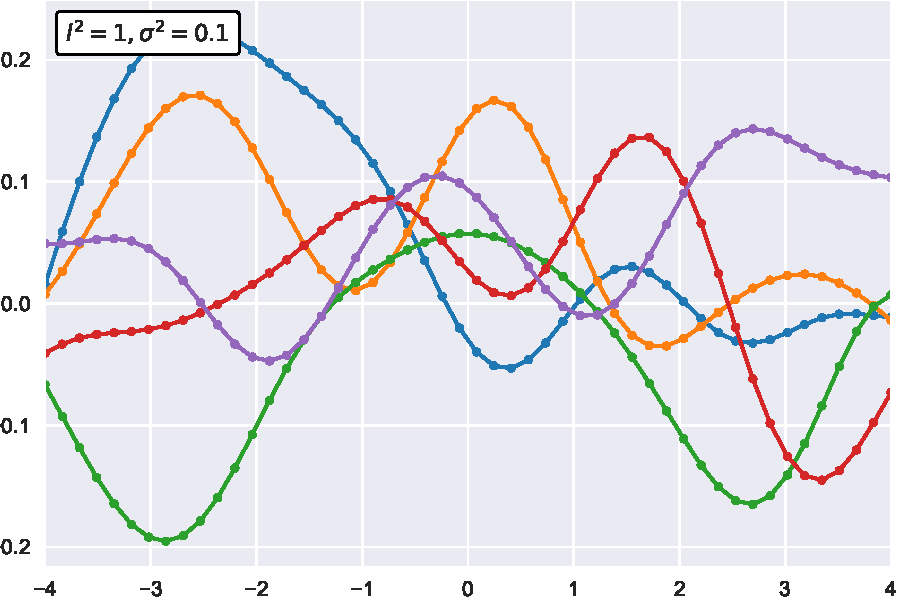
\includegraphics[width=\linewidth]{images/Gaussian process/RBF - sigma=01.pdf}
  \caption{$\sigma^2=0.1$}
\end{subfigure}%
\begin{subfigure}{.5\textwidth}
  \centering
  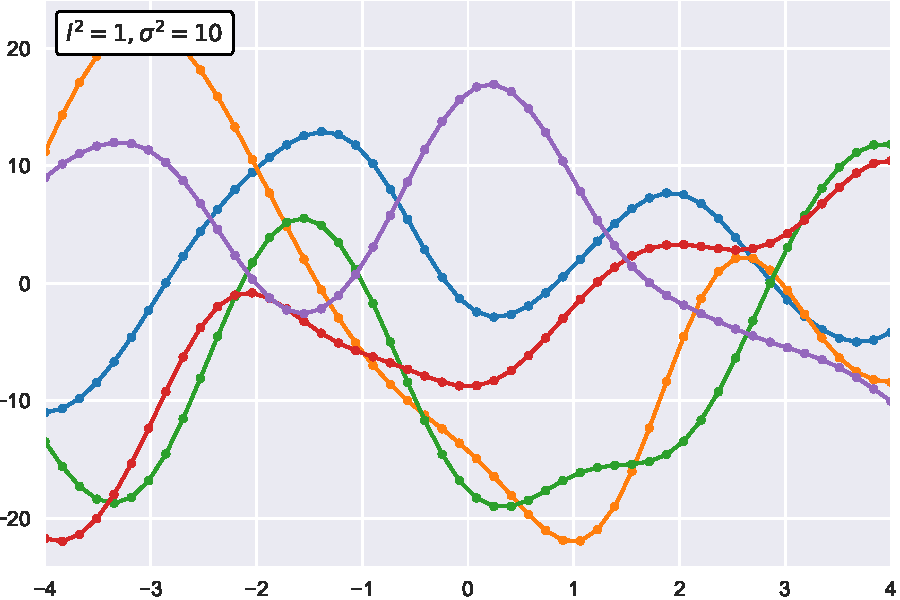
\includegraphics[width=\linewidth]{images/Gaussian process/RBF - sigma=10.pdf}
  \caption{$\sigma^2=10$}
\end{subfigure}
\caption{Graph of functions with distribution $f\sim \mathcal{GP}(\bm{0},k)$ where $k(x,x')$ is the squared-exponential kernel and $l^2=1$, parameter $\sigma^2$ is varied. Code \ref{RBF - sigma}.}
\label{10 sample exponential modified sigma}
\end{figure}

In the two cases, therefore, it changes how far the functions are from the line $x=0$, i.e. proportionally to the value of $\sigma^2$. In reality, $\sigma^2$ affects the tendency of the functions to distance themselves from the mean $m(x)$.

To understand the influence of the parameter $l^2$, graphs of functions with distribution $f\sim \mathcal{GP}(m,k)$ are shown below, where $m(x)=0$ and $k(x,x')$ is the squared-exponential kernel and the parameter $l^2$ is varied.


%%%%%%%%%%%%%%%%%%%%%%%%%%%%%%%%%%%
%%%%%% IMMAGINI: PARAMETRO l
%%%%%%%%%%%%%%%%%%%%%%%%%%%%%%%%%%%
\begin{figure}[h]
\centering
\begin{subfigure}{.5\textwidth}
  \centering
  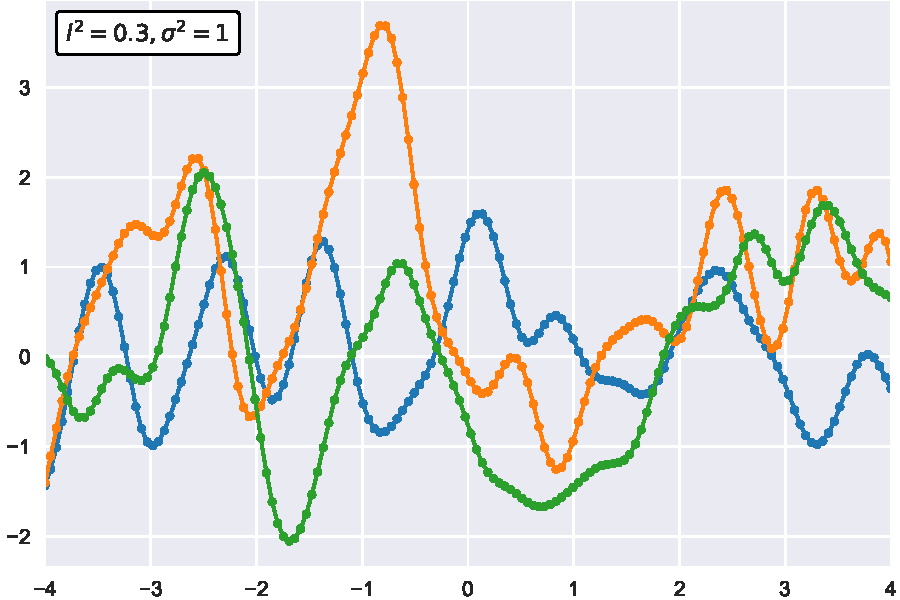
\includegraphics[width=\linewidth]{images/Gaussian process/RBF - l=03.pdf}
  \caption{$l^2=0.3$}
\end{subfigure}%
\begin{subfigure}{.5\textwidth}
  \centering
  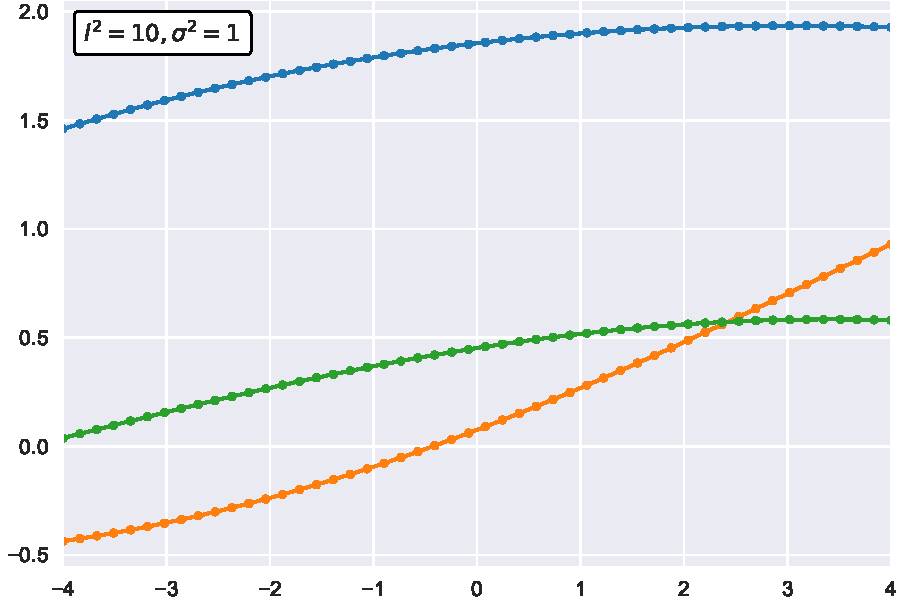
\includegraphics[width=\linewidth]{images/Gaussian process/RBF - l=10.pdf}
  \caption{$l^2=10$}
\end{subfigure}
\caption{Graph of functions with distribution  $f\sim \mathcal{GP}(\bm{0},k)$ where $k(x,x')$ is the squared-exponential kernel and $\sigma^2=1$, parameter $l^2$ is varied. Code \ref{codice9}.}
\label{10 sample exponential modified l}
\end{figure}

The parameter $l^2$ thus modifies the oscillation frequency of the functions.

\newpage

To understand the influence of the mean function, graphs of functions with distribution $f\sim \mathcal{GP}(m,k)$ where $m(x)=x^3$ and $k(x,x')$ the squared-exponential kernel are shown below.
%%%%%%%%%%%%%%%%%%%%%%%%%
%%%%%%%%% IMMAGINE
%%%%%%%%%%%%%%%%%%%%%%%%
\begin{figure}[h]
    \centering
    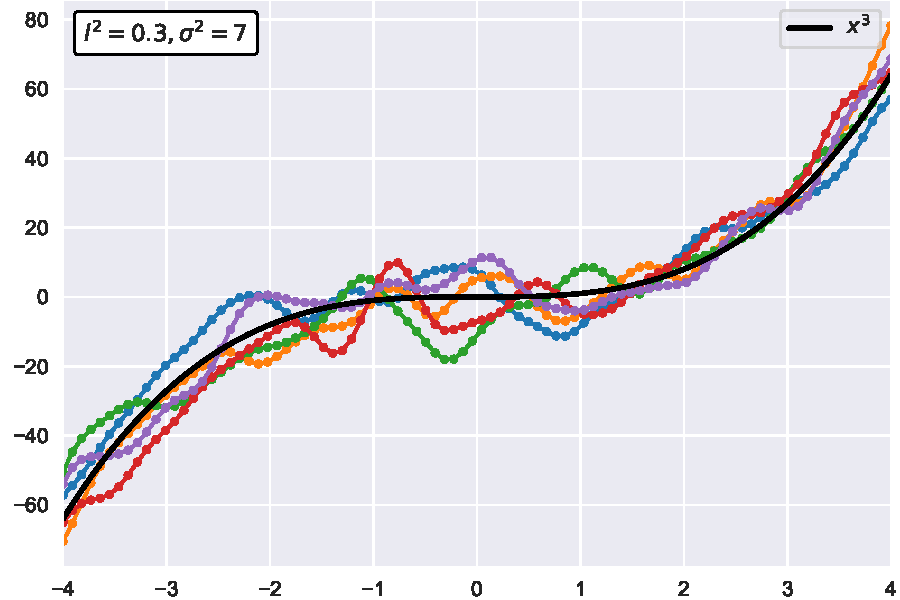
\includegraphics[width=0.85\textwidth]{images/Gaussian process/RBF - cubedmean.pdf}
    \caption{Graph of functions with distribution  $f\sim \mathcal{GP}(m,k)$ where $m(x)=x^3$ e $k(x,x')$ is the squared-exponential kernel, $\sigma^2=7$ and $l=0.3$. Code \ref{codice10}.}
    \label{10 sample exponential kernel cubed mean}
\end{figure}

Parameters have been chosen so that the graphs of the functions stand out. With $\sigma^2=7$ (thus a large distance from the mean function) and $l^2=0.3$ (thus a large oscillation frequency) the functions tend to emulate the mean $m(x)=x^3$ while maintaining the kernel-induced properties.

\newpage








\newpage

\subsection{Periodic kernel}

%%%%%%%%%%%%%%%%%%%%%%%%%%%%
%%%%%%%%% PERIODIC
%%%%%%%%%%%%%%%%%%%%%%%%%%%%
\begin{defi}[Periodic kernel]
  The \textbf{periodic kernel} has form:
\[
k(x,x')=\sigma^2 \text{exp}\left( -\frac{2}{l^2} \text{sin}^2\left( \pi \frac{|x-x'|}{p}\right)\right).
\]
This kernel is therefore also isotropic.
\end{defi}

The graph of the function $k(x,x')$ is shown. Note that the parameter $\sigma^2$ affects the peak of the function as in the \textit{squared-esponential kernel}, similarly the parameter $l^2$ affects the function as in the previous kernel, the parameter $p$ affects the periodicity of the kernel. 


%%%%%%%%%%%%%%%%%%%%%%%%%
%%%%%%%%% IMMAGINE
%%%%%%%%%%%%%%%%%%%%%%%%
\begin{figure}[h]
    \centering
    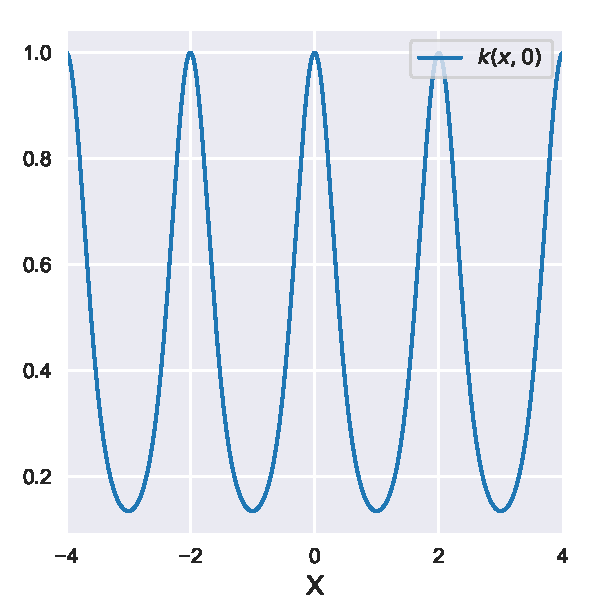
\includegraphics[width=0.6\textwidth]{images/Gaussian process/Periodic kernel.pdf}
    \caption{Graph of $k(x,x')$ periodic kernel, $\sigma^2=1$, $l^2=1$, $p=2$. Code \ref{periodic Kernel}.}
    \label{periodic kernel}
\end{figure}




\newpage
Graphs of functions with distribution $f\sim \mathcal{GP}(m,k)$ where $m(x)=0$ and $k(x,x')$ is the periodic kernel are shown below.

%%%%%%%%%%%%%%%%%%%%%%%%%
%%%%%%%%% IMMAGINE
%%%%%%%%%%%%%%%%%%%%%%%%
\begin{figure}[h]
    \centering
    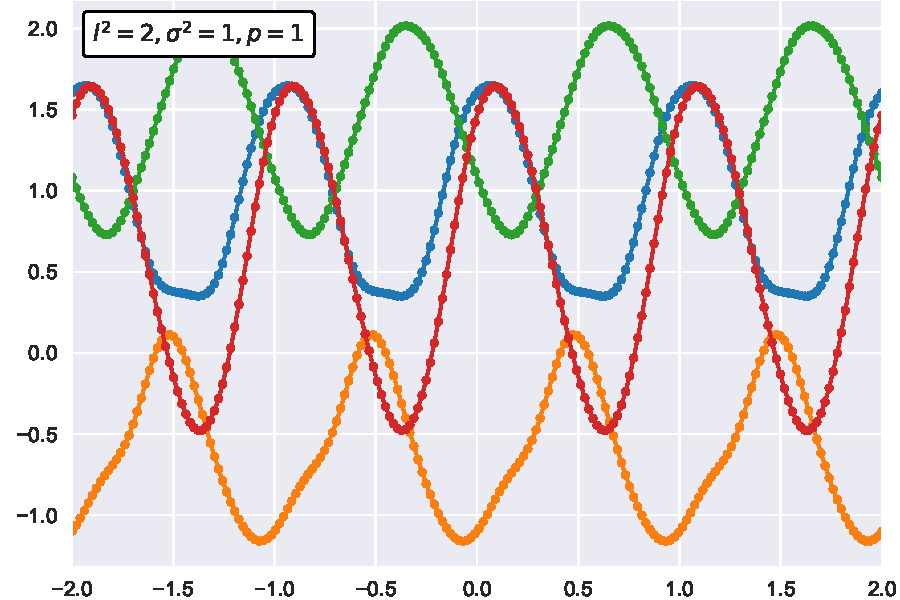
\includegraphics[width=0.85\textwidth]{images/Gaussian process/Periodic sample.pdf}
    \caption{Graph of functions with distribution  $f\sim \mathcal{GP}(\bm{0},k)$ where $k(x,x')$ is the periodic kernel and $\sigma^2=1$, $l^2=2$, $p=1$. Code \ref{periodic sample}.}
    \label{3 sample periodic kerne zero mean}
\end{figure}

As the name of the kernel suggests, the functions are periodic.
To understand the influence of the parameter $\sigma^2$, graphs of functions with distribution $f\sim \mathcal{GP}(m,k)$ where $m(x)=0$ and $k(x,x')$ is the periodic kernel and the parameter $\sigma^2$ is varied are shown below.

%%%%%%%%%%%%%%%%%%%%%%%%%%%%%%%%%%%
%%%%%% IMMAGINI: PARAMETRO sigma
%%%%%%%%%%%%%%%%%%%%%%%%%%%%%%%%%%%
\begin{figure}[h]
\centering
\begin{subfigure}{.5\textwidth}
  \centering
  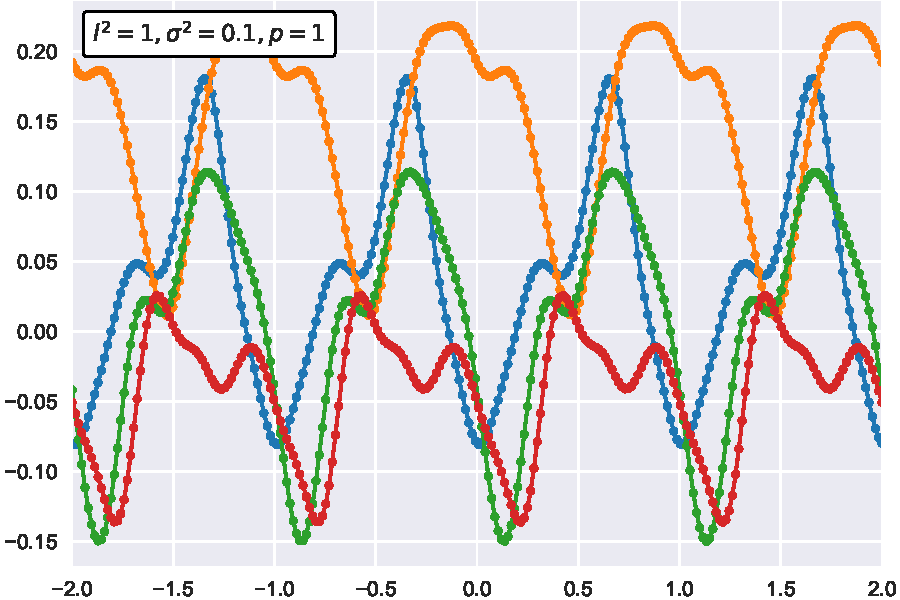
\includegraphics[width=\linewidth]{images/Gaussian process/Periodic - sigma=01.pdf}
  \caption{$\sigma^2=0.1$}
\end{subfigure}%
\begin{subfigure}{.5\textwidth}
  \centering
  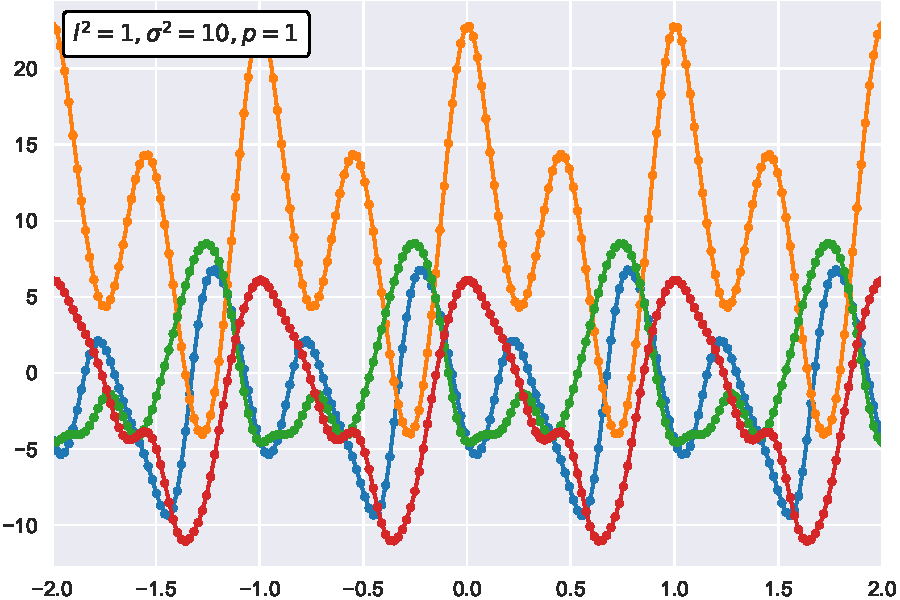
\includegraphics[width=\linewidth]{images/Gaussian process/Periodic - sigma=10.pdf}
  \caption{$\sigma^2=10$}
\end{subfigure}
\caption{Graph of functions with distribution  $f\sim \mathcal{GP}(\bm{0},k)$ where $k(x,x')$ is the periodic kernel and $l^2=1, p=1$, parameter $\sigma^2$ is varied. Code \ref{Periodic sigma}.}
\label{10 sample periodic modified sigma}
\end{figure}

The parameter $\sigma^2$ is thus responsible for the shift of the functions away from the mean, exactly as for the squared-exponential kernel (the figure \ref{10 sample exponential modified sigma} shows similar results).


\newpage

To understand the influence of parameter $p$, graphs of functions with distribution $f\sim \mathcal{GP}(m,k)$ where $m(x)=0$ and $k(x,x')$ is the periodic kernel and parameter $p$ is varied are shown below.

%%%%%%%%%%%%%%%%%%%%%%%%%%%%%%%%%%%
%%%%%% IMMAGINI: PARAMETRO p
%%%%%%%%%%%%%%%%%%%%%%%%%%%%%%%%%%%
\begin{figure}[h]
\centering
\begin{subfigure}{.5\textwidth}
  \centering
  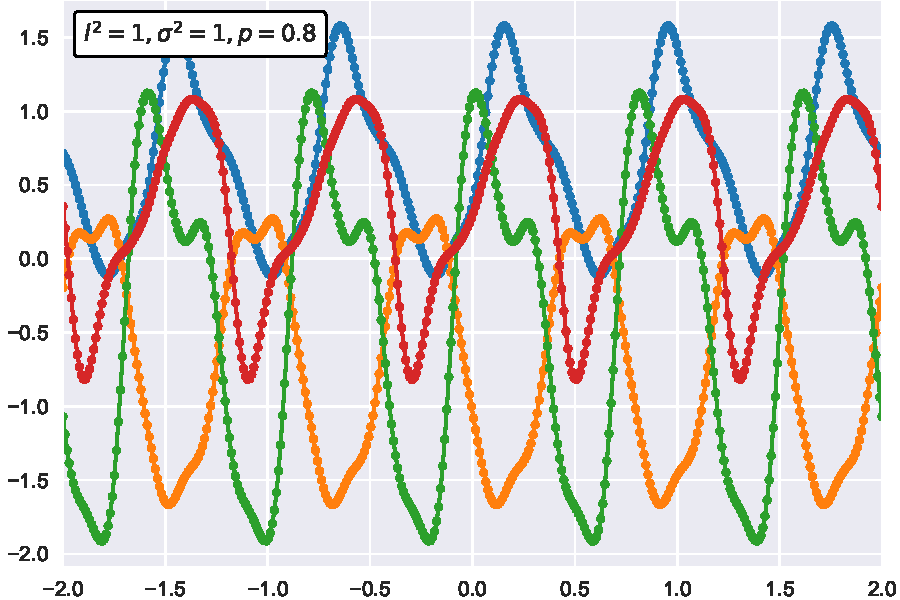
\includegraphics[width=\linewidth]{images/Gaussian process/Periodic - p=08.pdf}
  \caption{$p=0.8$}
\end{subfigure}%
\begin{subfigure}{.5\textwidth}
  \centering
  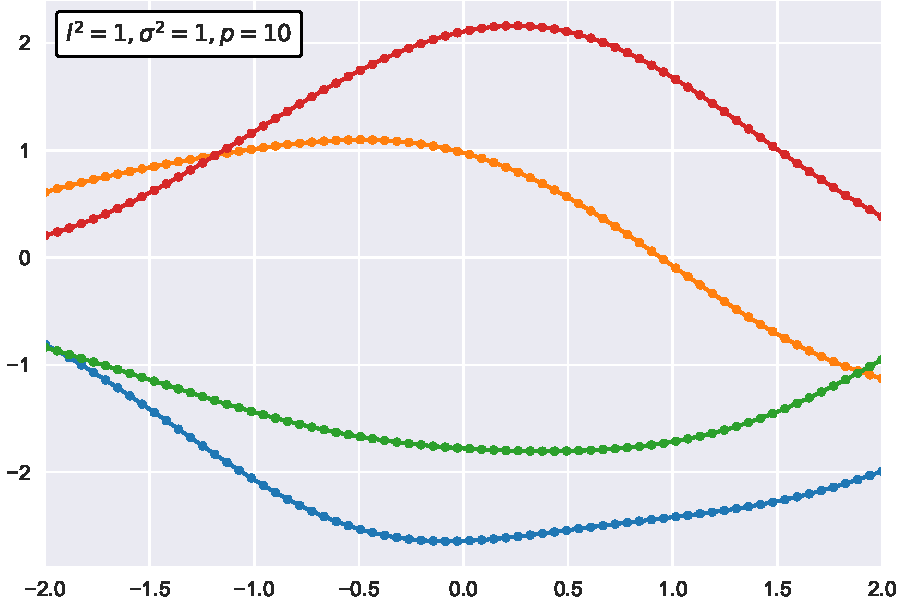
\includegraphics[width=\linewidth]{images/Gaussian process/Periodic - p=10.pdf}
  \caption{$p=10$}
\end{subfigure}
\caption{Graph of functions with distribution  $f\sim \mathcal{GP}(\bm{0},k)$ where $k(x,x')$ is the periodic kernel and $\sigma^2=1$, $l^2=1$ and parameter $p$ is varied. Code \ref{periodic p}.}
\label{10 sample periodic modified p}
\end{figure}

The parameter $p$ thus influences the period of the functions.

To understand the influence of parameter $l^2$, graphs of functions with distribution $f\sim \mathcal{GP}(m,k)$ are shown below, where $m(x)=0$ and $k(x,x')$ is the periodic kernel and parameter $l^2$ is varied.

%%%%%%%%%%%%%%%%%%%%%%%%%%%%%%%%%%%
%%%%%% IMMAGINI: PARAMETRO l
%%%%%%%%%%%%%%%%%%%%%%%%%%%%%%%%%%%
\begin{figure}[h]
\centering
\begin{subfigure}{.5\textwidth}
  \centering
  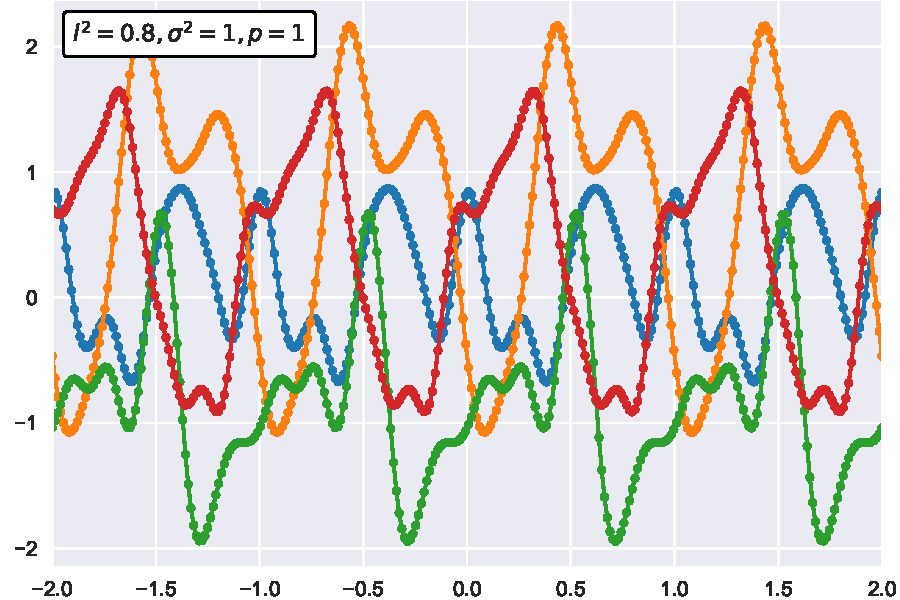
\includegraphics[width=\linewidth]{images/Gaussian process/Periodic - l=0.8.pdf}
  \caption{$l^2=0.8$}
\end{subfigure}%
\begin{subfigure}{.5\textwidth}
  \centering
  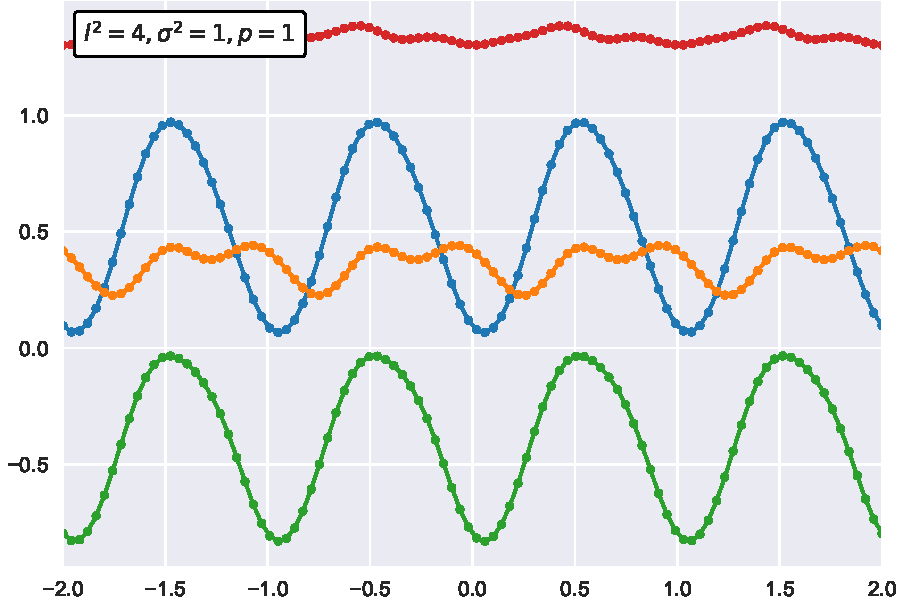
\includegraphics[width=\linewidth]{images/Gaussian process/Periodic - l=4.pdf}
  \caption{$l^2=4$}
\end{subfigure}
\caption{Graph of functions with distribution  $f\sim \mathcal{GP}(\bm{0},k)$ where $k(x,x')$ is the periodic kernel and $\sigma^2=1$, $p=1$ and parameter $l^2$ is varied. Code \ref{periodic l}.}
\label{10 sample periodic modified l}
\end{figure}

The parameter $l^2$ thus influences the 'smoothness' of the frequency of the functions.


\newpage 
To understand the influence of the mean function, graphs of functions with distribution $f\sim \mathcal{GP}(m,k)$ where $m(x)=x^3$ and $k(x,x')$ the periodic kernel are shown below.
%%%%%%%%%%%%%%%%%%%%%%%%%
%%%%%%%%% IMMAGINE
%%%%%%%%%%%%%%%%%%%%%%%%
\begin{figure}[h]
    \centering
    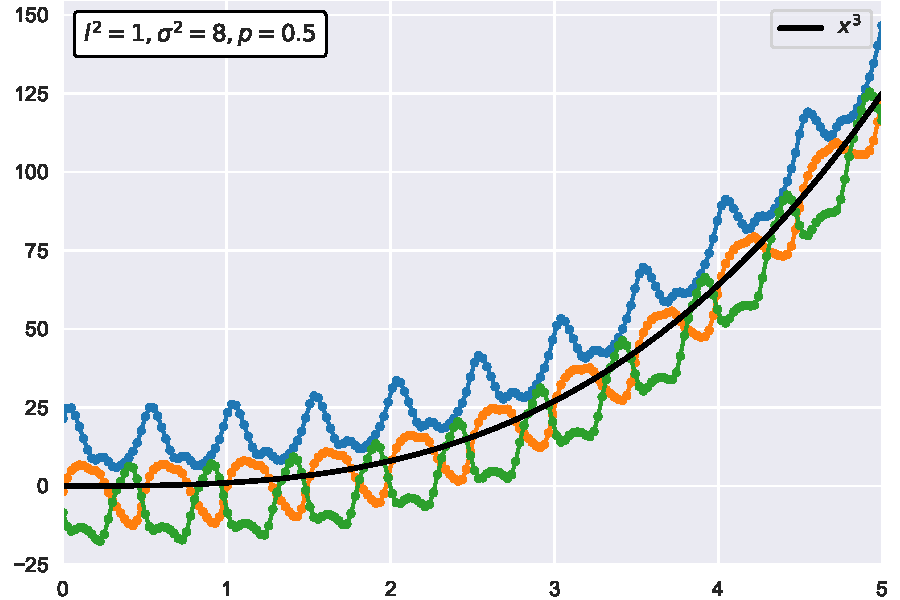
\includegraphics[width=0.85\textwidth]{images/Gaussian process/Periodic - cubedmean.pdf}
    \caption{Graph of functions with distribution  $f\sim \mathcal{GP}(m,k)$ where $m(x)=x^3$ and $k(x,x')$ the periodic kernel, $\sigma^2=8$, $l^2=1$ and $p=0.5$. Code \ref{priodic cubedmean}.}
    \label{3 sample periodic kernel cubed mean}
\end{figure}

Parameters have been chosen so that the graphs of the functions stand out. With $\sigma^2=8$ (thus a large distance from the mean function) and $p=0.5$ (thus a large oscillation frequency) and $l^2=1$ (thus very "angular") the functions tend to emulate the mean $m(x)=x^3$ while maintaining the kernel-induced properties.

\newpage



\subsection{Covariance function in more dimensions}\label{multidimensionalKernel}
One can extend covariance functions in multiple dimensions in various ways. Since the multi-dimensional extension is almost identical for each covariance function, the case of the squared-exponential kernel is shown, as it will be used in the training part of the paper.\\
In order to extend the squared-exponential kernel, it is necessary to extend the subtraction $x-x'$ in more dimensions. The simplest way is to consider the norm $||x-x'||$, a more flexible way is to consider $(x-x')^\text{T}M(x-x')$ where $M$ is a matrix.
This makes it possible to generalise the case:
\[
k(x,x')=\sigma^2 \text{exp}\left( -\frac{||x-x'||^2}{2l^2} \right),
\]
which can be obtained as:
\[
k(x,x')=\sigma^2 \text{exp}\left( -\frac{(x-x')^\text{T}M(x-x')}{2} \right)
\]
imposing $M=l^{-2}I$.\\
The matrix kernel structure allows each dimension to be given a different length scale $l_i$, imposing $M=\text{diag}(\bf{l})^{-2}$, where $\mathbf{l}=(l_1,...,l_n)^\text{T}$. This feature is crucial in training (discussed later in the paper) because if one of these $l_i$ becomes large, the corresponding dimension (which will be seen to correspond to a parameter to be optimised) "loses relevance". The image \ref{multidimensional} provides an example of such behaviour.

%%%%%%%%%%%%%%%%%%%%%%%%%
%%%%%%%%% IMMAGINE
%%%%%%%%%%%%%%%%%%%%%%%%
\begin{figure}[h]
    \centering
    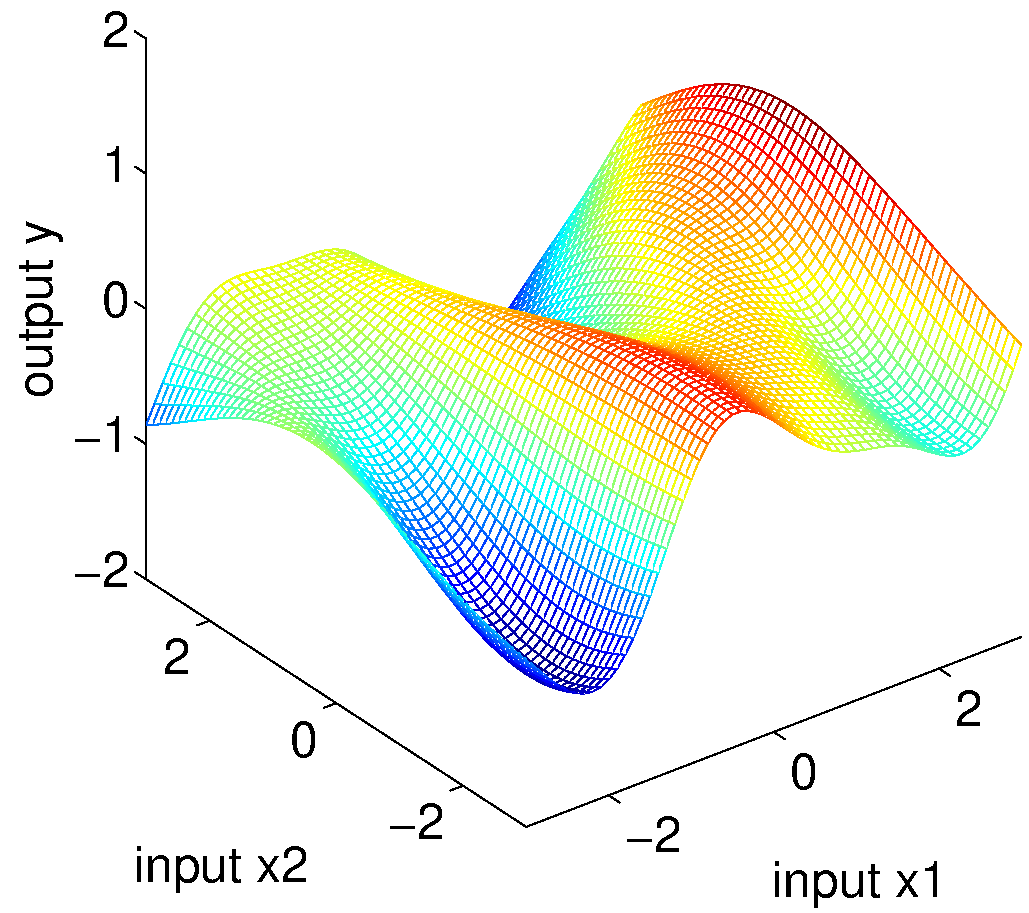
\includegraphics[width=0.6\textwidth]{images/Gaussian process/Multidimensional RBF.pdf}
    \caption{Graph of function with distribution $f\sim \mathcal{GP}(0,k)$ with $k(x,x')$ the squared-exponential kernel in two dimensions in which $M=\text{diag}(1,3)^{-2}$. The function tends to change faster along the $x_1$ direction than along the $x_2$ direction. \cite{murphy_machine_2012}}
    \label{multidimensional}
\end{figure}




\newpage

\subsection{Combining covariance functions}
In the previous sections, the influence of the covariance function on the shape of the function graph has been explained. However, it is not uncommon to have to use functions with shapes other than those imposed by the previously introduced covariance functions. In this case it is possible to construct a new kernel according to the proposition \ref{combining kernel}.


\begin{prop} \label{combining kernel}
  Given two kernels $K_1(x,x')$ and $K_2(x,x')$, by the properties of a kernel the following are still kernels:
\[
\begin{array}{l}
    K(x,x') = c\cdot K_1(x,x') \quad \forall c>0 \text{ costante}\\
    K(x,x') = f(x)K_1(x,x')f(x') \quad \forall f \text{ funzione}\\
    K(x,x') = q(K_1(x,x')) \quad \forall q \text{ funz. polin. a coeff. non negativi}\\
    K(x,x') = \text{exp}(K_1(x,x'))\\
    K(x,x') = K_1(x,x')+K_2(x,x')\\
    K(x,x') = K_1(x,x')\times K_2(x,x')\\
\end{array}
\]
\end{prop}
It is not in the interests of the paper to study in depth the possible combinations of kernels introduced; however, two simple cases of kernel combinations are given for illustrative purposes only.

\newpage




\subsubsection{Squared exponential + periodic kernel}


%%%%%%%%%%%%%%%%%%%%%%%%%
%%%%%%%%% IMMAGINE
%%%%%%%%%%%%%%%%%%%%%%%%
\begin{figure}[h]
    \centering
    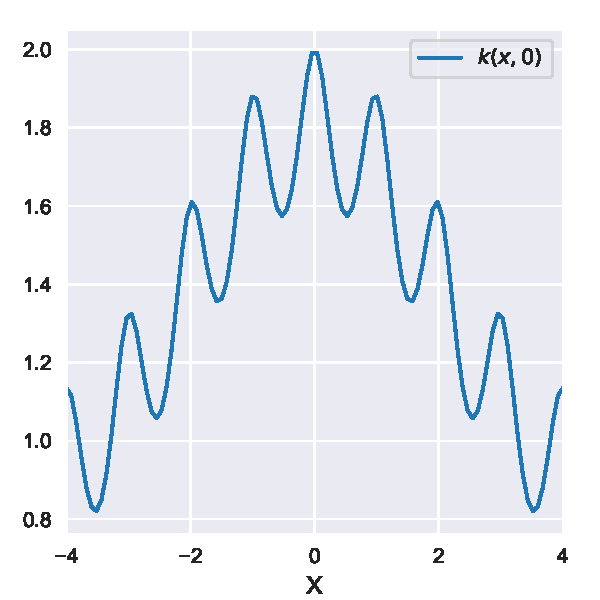
\includegraphics[width=0.55\textwidth]{images/Gaussian process/RBF + periodic kernel.pdf}
    \caption{Graph of $k(x,x')$ squared-exponential kernel summed to periodic kernel. $\sigma^2=1$, $l=2$, $p=1$. Code \ref{RBF + periodic kernel}.}
    \label{SE + periodic kernel}
\end{figure}



%%%%%%%%%%%%%%%%%%%%%%%%%
%%%%%%%%% IMMAGINE
%%%%%%%%%%%%%%%%%%%%%%%%
\begin{figure}[h]
    \centering    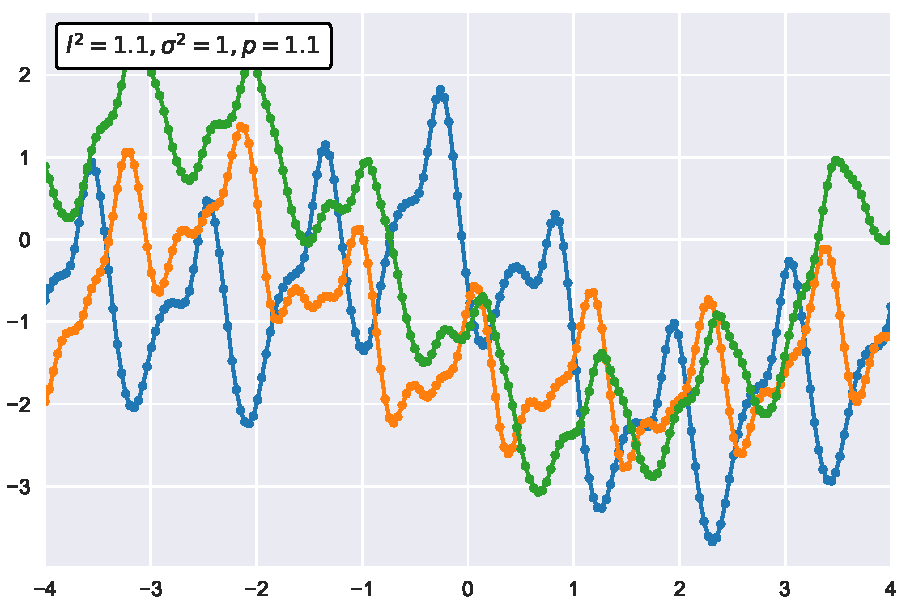
\includegraphics[width=0.69\textwidth]{images/Gaussian process/RBF + periodic sample.pdf}
    \caption{Graph of functions with distribution  $f\sim \mathcal{GP}(\bm{0},k)$ where $k(x,x')$ is the squared-exponential summed to periodic kernel and $l^2=1.1$, $\sigma^2=1$, $p=1.1$. Code \ref{RBF + periodic sample}.}
    \label{SE + periodic sample}
\end{figure}

Combining the two kernels therefore generates periodic functions with perturbations on the pair of axes.

\newpage

\subsubsection{Linear $\times$ linear kernel}

%%%%%%%%%%%%%%%%%%%%%%%%%
%%%%%%%%% IMMAGINE
%%%%%%%%%%%%%%%%%%%%%%%%
\begin{figure}[h]
    \centering
    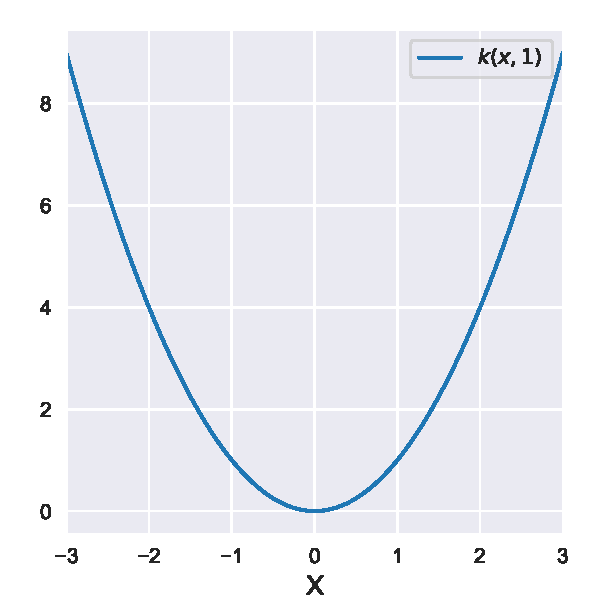
\includegraphics[width=0.55\textwidth]{images/Gaussian process/Linear x Linear kernel.pdf}
    \caption{Graph of $k(x,x')$ linear kernel multiplied by linear kernel. $\sigma_b^2=0$, $\sigma_v^2=1$, $c=0$, $x'=1$. Code \ref{linear x linear}.}
    \label{linear * linear kernel}
\end{figure}


%%%%%%%%%%%%%%%%%%%%%%%%%
%%%%%%%%% IMMAGINE
%%%%%%%%%%%%%%%%%%%%%%%%
\begin{figure}[h]
    \centering
    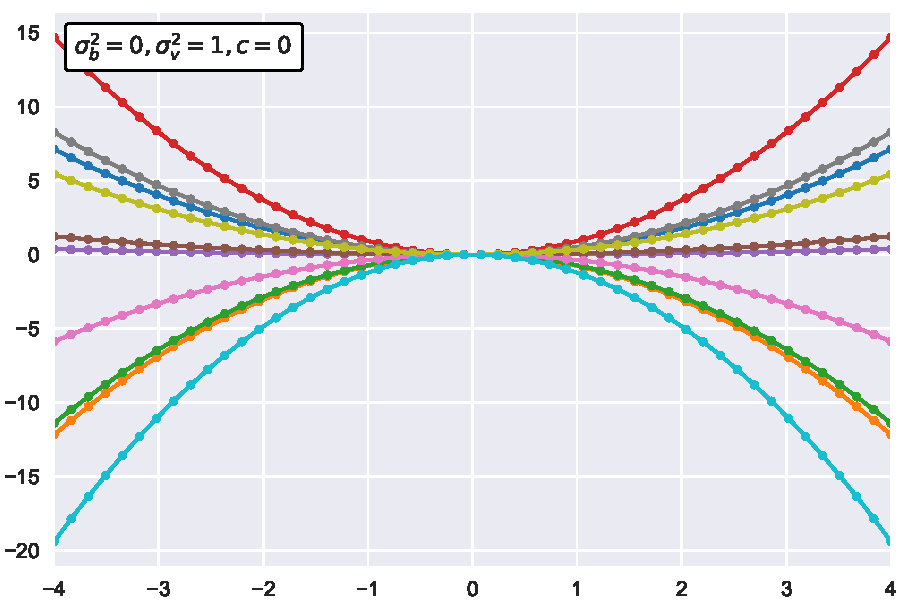
\includegraphics[width=0.68\textwidth]{images/Gaussian process/linear x linear sample.pdf}
    \caption{Graph of functions with distribution  $f\sim \mathcal{GP}(\bm{0},k)$ where $k(x,x')$ is the linear kernel multiplied by linear kernel and $\sigma_b^2=0$, $\sigma_v^2=1$, $c=0$. Code \ref{linear x linear sample}.}
    \label{linear * linear sample}
\end{figure}


Combining the two kernels therefore generates functions with parabolic behaviour. In a sense, it was possible to predict this result by remembering that the linear kernel generates straight lines.

\newpage



\subsubsection{Real-life example of a compound covariance function}\label{section: mauna loa}
It is taken from \cite{rasmussen_gaussian_2006} an example of a regression in which several kernel functions need to be composed.  The data consist of monthly mean atmospheric $CO_2$ concentrations (in parts per million volume: $ppmv$) derived from air samples collected at the Mauna Loa Observatory in Hawaii between 1958 and 2003 (with some missing values). The objective is to model the concentration of $CO_2$ as a function of time $x$, i.e. to predict what is known as \textit{Keeling's curve}. From the figure \ref{CO2}, some features are evident: a long-term increasing trend, a pronounced seasonal variation and some minor irregularities. 


%%%%%%%%%%%%%%%%%%%%%%%%%
%%%%%%%%% IMMAGINE
%%%%%%%%%%%%%%%%%%%%%%%%
\begin{figure}[ht]
    \centering
    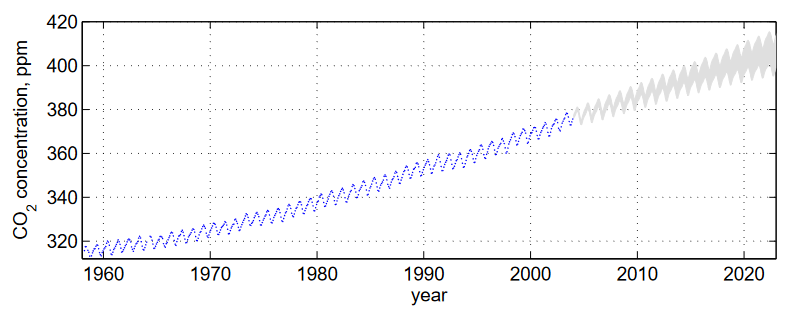
\includegraphics[width=1\textwidth]{images/Gaussian process/Co2_example.PNG}
    \caption{545 observations of monthly averages of the atmospheric concentration of $CO_2$ between 1958 and 2003, the $95\%$ confidence region for a 20-year Gaussian process regression model in the future is also shown. \cite{rasmussen_gaussian_2006}}
    \label{CO2}
\end{figure}


A squared-exponential kernel is used to model the regular and increasing long-term trend:
\[
k_1(x,x')=\theta_1^2\text{exp}\left(-\frac{(x-x')^2}{2\theta_2^2}\right).
\]


The periodic kernel with a period of one year is used to model seasonal variation. Since the seasonal trend is not exactly periodic, the product with a squared-exponential kernel is considered to allow for a decay that is not exactly periodic: 
\[
k_2(x, x') = \theta^2_3 \text{exp}\left( - \frac{(x - x')^2}{2\theta^2_4} - \frac{2 \text{sin}^2(\pi(x - x'))}{\theta^2_5} \right).
\]
A \textit{rational quadratic} kernel is used to model the (small) medium-term irregularities (not introduced in the paper): 
\[
k_3(x, x') = \theta^2_6 \left( 1 + \frac{(x - x')^2}{2\theta_8\theta^2_7} \right)^{-\theta_8}.
\] 
Finally, noise is modelled as the sum of a squared-exponential contribution and an independent component:
\[
k_4(x_p, x_q) = \theta^2_9 \text{exp}\left( \frac{- (x_p - x_q)^2}{2\theta^2_{10}} \right) + \theta^2_{11} \delta_{pq}.
\]

The overall kernel results:
\[
k(x,x')=k_1(x,x')+k_2(x,x')+k_3(x,x')+k_4(x,x'),
\]
where we have $\bm{\theta}=(\theta_1,...,\theta_{11})$ hyperparameters\footnote{see \ref{gerarchica}.}. After a training phase of the model, values are given to the $\theta_i$\footnote{It is explained how this is done in the chapter \ref{machineLearning}.}. Figure \ref{CO2} shows how the model predicts the trend of the atmospheric concentration of $CO_2$ over the twenty years since the last measurement, also showing the ninety-five per cent confidence region. It can be seen that the further one goes in time, the wider the confidence region becomes.\\
Intuitively, the model seems to follow the trend of the graph well, although as the years go by, the region of uncertainty becomes larger, informing little about the actual concentration of $CO_2$. Figure \ref{CO2_comparison} compares the model's prediction with actual data taken from the \href{https://gml.noaa.gov/ccgg/trends/}{Global Monitoring Laboratory}.


%%%%%%%%%%%%%%%%%%%%%%%%%
%%%%%%%%% IMMAGINE
%%%%%%%%%%%%%%%%%%%%%%%%
\begin{figure}[h]
    \centering
    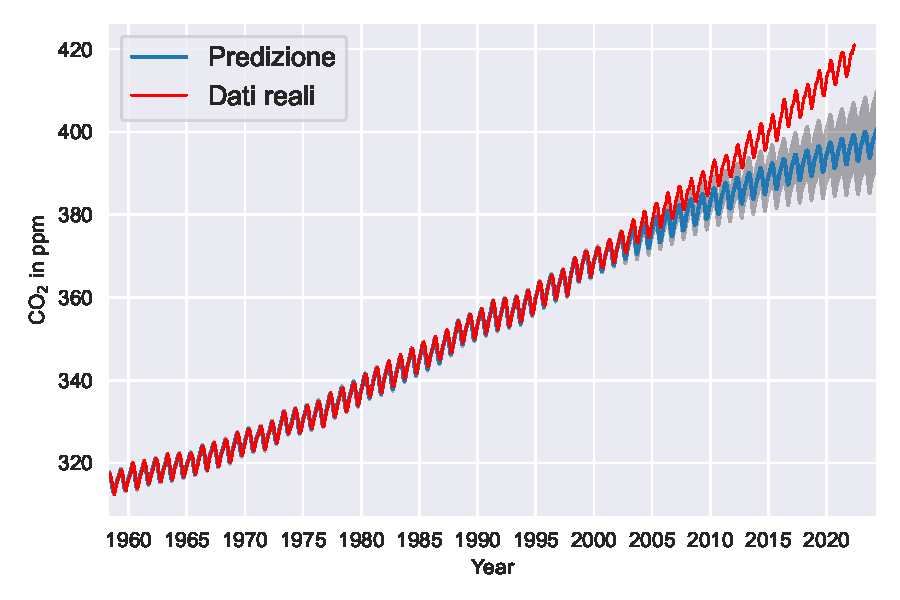
\includegraphics[width=1\textwidth]{images/Gaussian process/MaunaLoaPrediction.pdf}
    \caption{Comparison of the prediction of $CO_2$ concentration with actual data until May 2022.}
    \label{CO2_comparison}
\end{figure}

\newpage

We can therefore see that the forecast was conservative in the long term: the large increase in the concentration of $CO_2$ is due, according to some sources, to how the flora has responded to climate change (drought and precipitation mainly), but also to the large emissions due to the use of fossil fuels.

In a way, therefore, it is reasonable that the prediction is not accurate in recent years as it should have predicted events (from climate change to different rates of fuel consumption) that were not present in the years when the Gaussian process 'learned'.

In figure \ref{CO2_comparison_zoomed}, the previous image from 1995 to 2022 is enlarged, thus emphasising the time period predicted by the Gaussian process.

It can be seen that after 2003, the prediction is rather inaccurate, failing to keep up with rapid human changes (in terms of pollution).  

%%%%%%%%%%%%%%%%%%%%%%%%%
%%%%%%%%% IMMAGINE
%%%%%%%%%%%%%%%%%%%%%%%%
\begin{figure}[h]
    \centering
    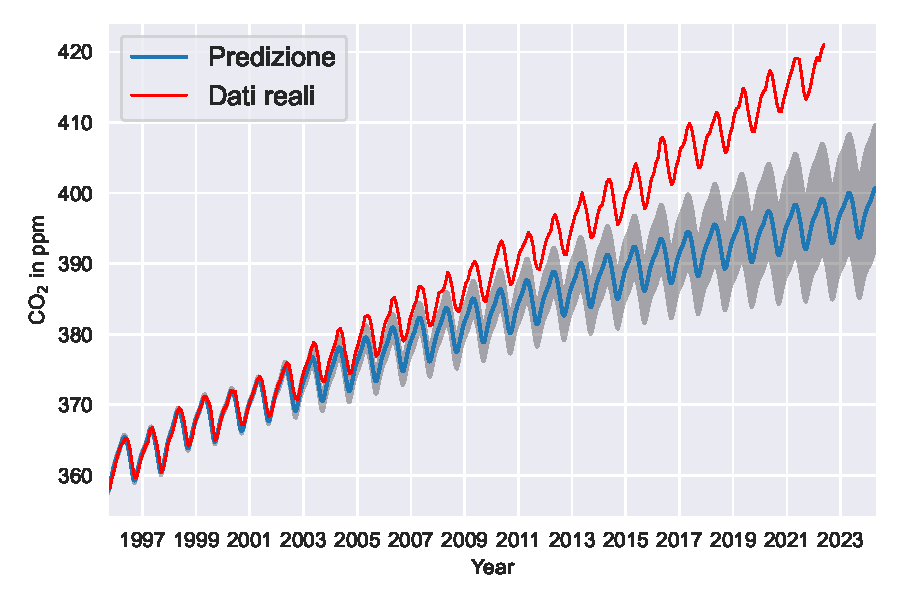
\includegraphics[width=1\textwidth]{images/Gaussian process/MaunaLoaPredictionZoom.pdf}
    \caption{Comparison of the prediction of $CO_2$ concentration with actual data up to 1995 to May 2022.}
    \label{CO2_comparison_zoomed}
\end{figure}




\newpage



\section{Predictions with noiseless observations}\label{regressioneGP}
This section explains how to exploit the information provided by \textit{training data} to generate a function that incorporates a priori knowledge in the case of observations without noise. \\


\begin{defi}[Noise-free training set]
  The \textbf{noise-free training set} is the set of observations \textit{noise-free} defined as: $ \mathcal{D}=\{ (x_n,y_n) : n=1,...,N\}$ where $y_n=f(x_n)$ is the observed value of the function $f$ at point $x_n$. 
\end{defi}


The purpose of the (noise-free) training set is to define a set of points $\mathcal{P}=\{x_n: n=1,...,N\}$ of which the value of the function is known in order to require the Gaussian process to generate functions that interpolate this set of points (i.e. that have value $y_n$ on every $x_n \in \mathcal{P}$ without uncertainty).

\begin{defi}[Test set]
  the \textbf{test set} is the set of values $X_*=\{x_n:n=1,...,N^*\}$ of which the prediction, i.e. the output of the function, is desired.
\end{defi}

Pragmatically, what is being done by defining the \textit{training set} $\mathcal{D}$ is to add the points of $\mathcal{P}$ to the set of points on which to evaluate the covariance function to construct the covariance matrix\footnote{As mentioned in \ref{footnote 1}, to obtain a graph it is necessary to start from a finite domain. This is why we speak of \textit{covariance matrix}.}. Through the conditioning process we obtain the \textit{a posteriori} distribution, that is, the distribution of the functions that interpolate the points of the training set, as illustrated in Figure \ref{intuitiveExplanationOfConditioning}.


%%%%%%%%%%%%%%%%%%%%%%%%%
%%%%%%%%% IMMAGINE
%%%%%%%%%%%%%%%%%%%%%%%%
\begin{figure}[h]
    \centering
    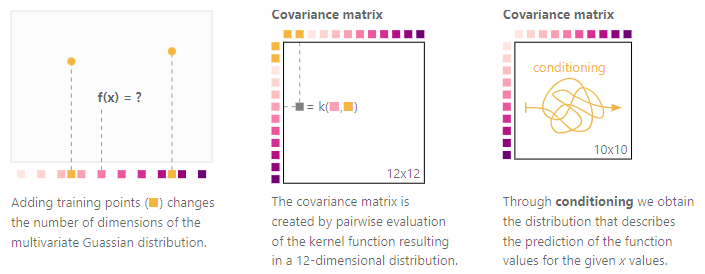
\includegraphics[width=1\textwidth]{images/Gaussian process/GPposterior.PNG}
    \caption{Graphical explanation of how a priori knowledge is incorporated \cite{gortler_visual_2019}.}
    \label{intuitiveExplanationOfConditioning}
\end{figure}

\newpage
Consider now a function distributed as $f\sim \mathcal{GP}(m,k)$. 
Consider now $X^*=\{x_i^*:i=1,\dots,N^*\}$ a \textit{test set} Of which you want to predict the outputs $\bm{f^*}=\left[f(x^*_1), \dots, f(x^*_{N^*}) \right]$; Let also  $\bm{f}=\left[f(x_1), \dots, f(x_N) \right]$ the outputs of the training set where $x_i\in \mathcal{P}$. Recalling that the outputs of the function $f$ follow a Gaussian distribution, the joint distribution can be derived:
\[
\begin{pmatrix}
\bm{f}\\
\bm{f^*}
\end{pmatrix}
=
\mathcal{N}\left(
\begin{pmatrix}
\bm{\mu}\\
\bm{\mu_*}
\end{pmatrix},
\begin{pmatrix}
\bm{K}_{X,X} & \bm{K}_{X,X^*}\\
\bm{K}_{X^*,X} & \bm{K}_{X^*,X^*}
\end{pmatrix}
\right)
\]

where $\bm{\mu}=\begin{pmatrix}m(x_1) \\ \vdots \\ m(x_N)\end{pmatrix}$, $\bm{\mu_*}=\begin{pmatrix}m(x^*_1) \\ \vdots \\ m(x^*_{N^*})\end{pmatrix}$, $\bm{K}_{X,X}=k(X,X)$ is a $N\times N^*$ matrix, $\bm{K}_{X,X^*}=k(X,X^*)$ is a $N\times N^*$ matrix, $\bm{K}_{X^*,X}=k(X^*,X)$ is a $N^*\times N^*$ matrix, $\bm{K}_{X^*,X^*}=k(X^*,X^*)$ is a $N^*\times N^*$ matrix .\\

From the proposition \ref{marginale-condizionata} we derive the conditional distribution of $\bm{f^*} | X^*, \mathcal{D}$:

\[
\bm{f^*} | X^*, \mathcal{D} \sim \mathcal{N}(\bm{\mu^*}, \bm{\Sigma^*})
\]

where:
\[
\begin{split}
\bm{\mu^*}=m(X^*)+\bm{K}_{X,X^*}^\text{T}\bm{K}^{-1}_{X,X}(\bm{f}-m(X))\\
\bm{\Sigma^*}=\bm{K}_{X^*,X^*}-\bm{K}_{X,X^*}^\text{T}\bm{K}^{-1}_{X,X}\bm{K}_{X,X^*}
\end{split}
\]


\newpage 
A graphical example of six-point interpolation is shown in Figure \ref{Interpolation}.


%%%%%%%%%%%%%%%%%%%%%%%%%
%%%%%%%%% IMMAGINE
%%%%%%%%%%%%%%%%%%%%%%%%
\begin{figure}[h]
    \centering
    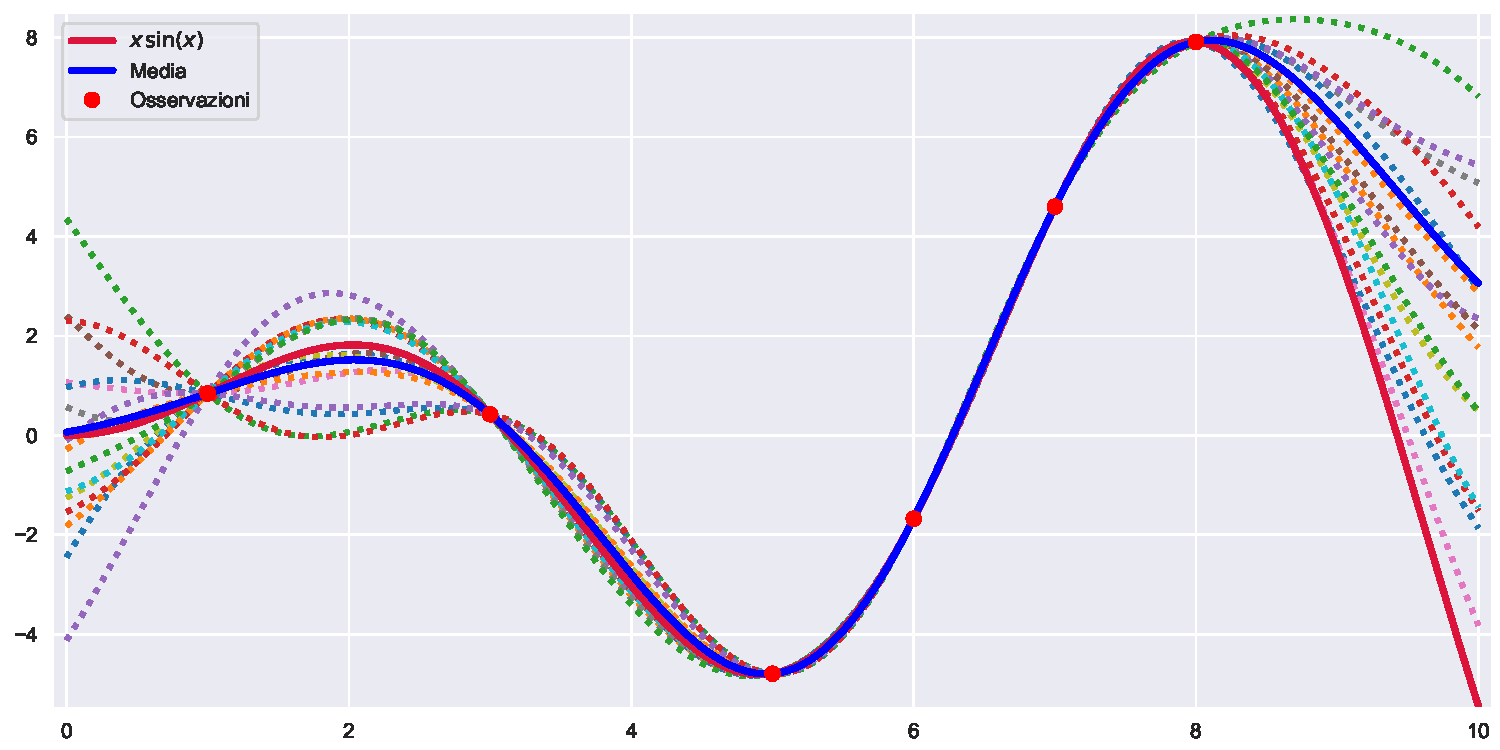
\includegraphics[width=1\textwidth]{images/Gaussian process/Noise-free - mean&f(x).pdf}
    \caption{Graph of functions with distribution $f\sim \mathcal{GP}(\bm{0},k)$ dove $k(\cdot,\cdot)$ is the squared-exponential kernel; the Gaussian process was conditioned to interpolate six points. Shown in red is the function from which the points to be interpolated were chosen, in blue the mean of the conditioned Gaussian process, as dashed lines some samples of the Gaussian process. Code \ref{interpolation code}.}
    \label{Interpolation}
\end{figure}

The mean of the conditional Gaussian process to interpolate the six points is the most reliable in predicting the function $x\cdot sin(x)$ from which the points to be interpolated were generated. The functions with distribution the conditional Gaussian process all have the property of interpolating the aforementioned points, however, in the rest of the plane they are more easily distanced from the mean, although they tend to stay in its vicinity. In Figure \ref{Interpolation confidence region} information from the a posteriori covariance matrix is exploited to draw the 95\% confidence region, within which most of the samples reside.


\newpage
%%%%%%%%%%%%%%%%%%%%%%%%%
%%%%%%%%% IMMAGINE
%%%%%%%%%%%%%%%%%%%%%%%%
\begin{figure}[h]
    \centering
    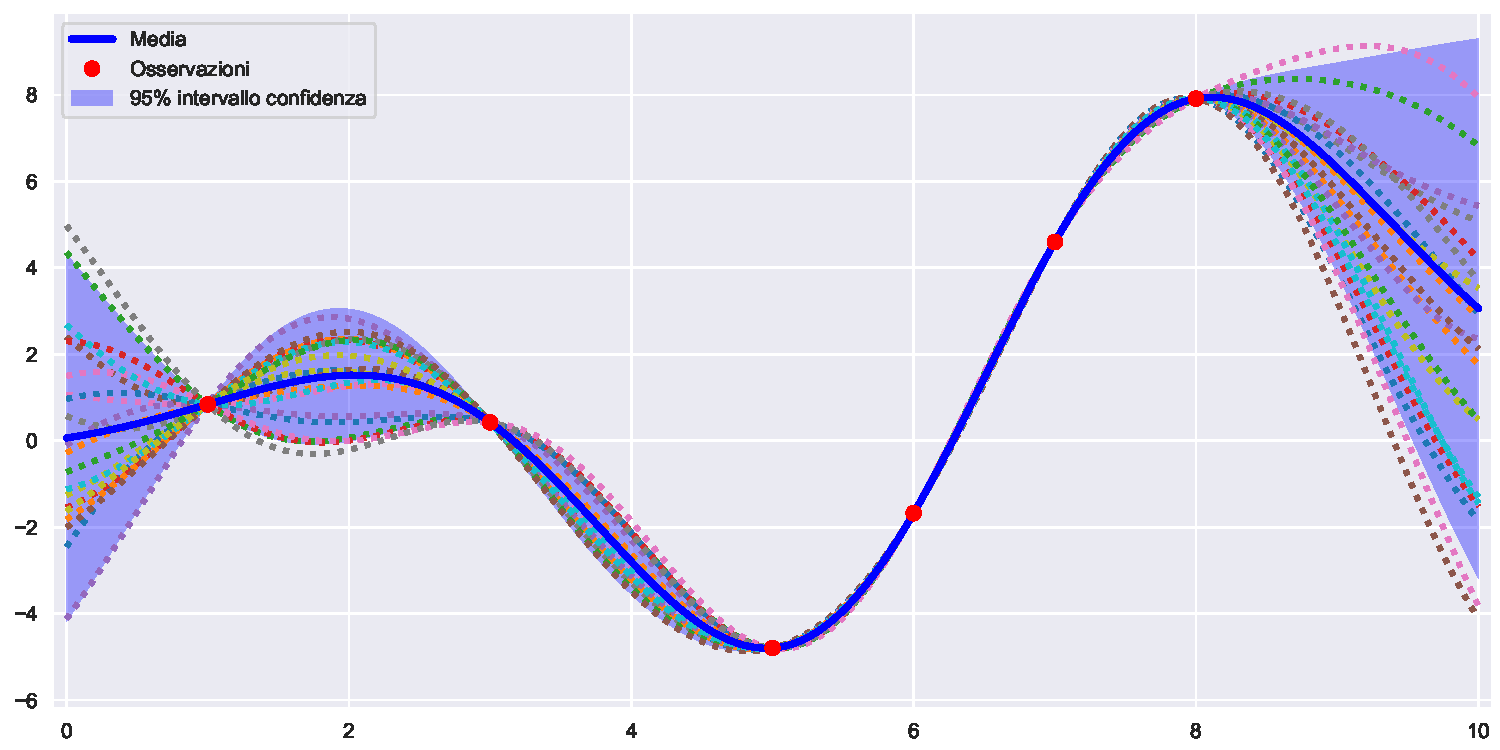
\includegraphics[width=1\textwidth]{images/Gaussian process/Noise-free - mean&samples.pdf}
    \caption{Graph of functions with distribution $f\sim \mathcal{GP}(\bm{0},k)$ where $k(\cdot,\cdot)$ is the squared-exponential kernel; the Gaussian process was conditioned to interpolate six points. Shown in blue is the 95\% confidence region, in blue the mean of the conditional Gaussian process, and as dashed lines some samples. Code \ref{interpolation confidence region code}.}
    \label{Interpolation confidence region}
\end{figure}

As anticipated, within the area given by $\bm{\mu^*}(x_i)\pm 1.96\bm{\Sigma^*}(x_i,x_i)$ (95\% confidence region) reside most of the samples of the a posteriori distribution. The farther one moves away from the interpolated points, the more easily the functions deviate from the mean, tending to move out of the area of uncertainty, as observed, for example, in the area near $x=10$ in Figure \ref{Interpolation confidence region}.



\section{Predictions with noisy observations}\label{noisyPrediction}
This section explains how to exploit the information provided by \textit{training data} to generate a function that incorporates a priori knowledge in the case of observations with noise. \\

\begin{defi}[Noisy training set]
  The \textbf{noisy training set} is the set of \textit{noisy} observations (i.e., with an error component) defined as: $\mathcal{D}=\{(x_n,y_n): n=1,... ,N\}$ where $y_n=f(x_n)+\epsilon$ is the observed value of the function $f$ at the point $x_n$ with a noise component $\epsilon\sim \mathcal{N}(0,\sigma_n^2)$ independent and identically distributed. 
\end{defi}
In this case you have:
\[
\text{Cov}(y_p,y_q)=k(x_p,x_q)+\sigma_n^2 \delta_{pq},
\]
or equivalently:
\[
\text{Cov}(\mathbf{y})=k(X,X)+\sigma_n^2I.
\]

\newpage

A notation analogous to the \ref{regressioneGP} section is used: $X^*=\{x_i^*: i=1,\dots,N^*\}$ is the \textit{test set} whose outputs are to be predicted $\bm{f^*}=\left[f(x^*_1), \dots, f(x^*_{N^*}) \right]$; $\bm{y}=\left[f(x_1)+\epsilon, \dots, f(x_N)+\epsilon \right]$ the outputs of the training set. \\
We proceed as in the case of prediction with noiseless observations:
\[
\begin{pmatrix}
\bm{y}\\
\bm{f^*}
\end{pmatrix}
=
\mathcal{N}\left(
\begin{pmatrix}
\bm{\mu}\\
\bm{\mu_*}
\end{pmatrix},
\begin{pmatrix}
\bm{K}_{X,X}+\sigma_n^2I & \bm{K}_{X,X^*}\\
\bm{K}_{X^*,X} & \bm{K}_{X^*,X^*}
\end{pmatrix}
\right)
\]
It is derived:
\[
\bm{f^*} | X^*, \mathcal{D} \sim \mathcal{N}(\bm{\mu^*}, \bm{\Sigma^*})
\]
where:
\[
\begin{split}
\bm{\mu^*}=m(X^*)+\bm{K}_{X,X^*}^\text{T}(\bm{K}_{X,X}+\sigma_n^2I)^{-1}(\bm{y}-m(X))\\
\bm{\Sigma^*}=\bm{K}_{X^*,X^*}-\bm{K}_{X,X^*}^\text{T}(\bm{K}_{X,X}+\sigma_n^2I)^{-1}\bm{K}_{X,X^*}
\end{split}
\]


A graphic example of how a Gaussian process interprets information given by observations with noise to predict a function is shown in Figure \ref{Noisy}.
As might be expected, since the observations in this case are with noise, the Gaussian process needs more observations in order to predict the trend of the function. Since interpolation does not occur, the Gaussian process predicts the function with less accuracy.
%%%%%%%%%%%%%%%%%%%%%%%%%
%%%%%%%%% IMMAGINE
%%%%%%%%%%%%%%%%%%%%%%%%
\begin{figure}[h]
    \centering
    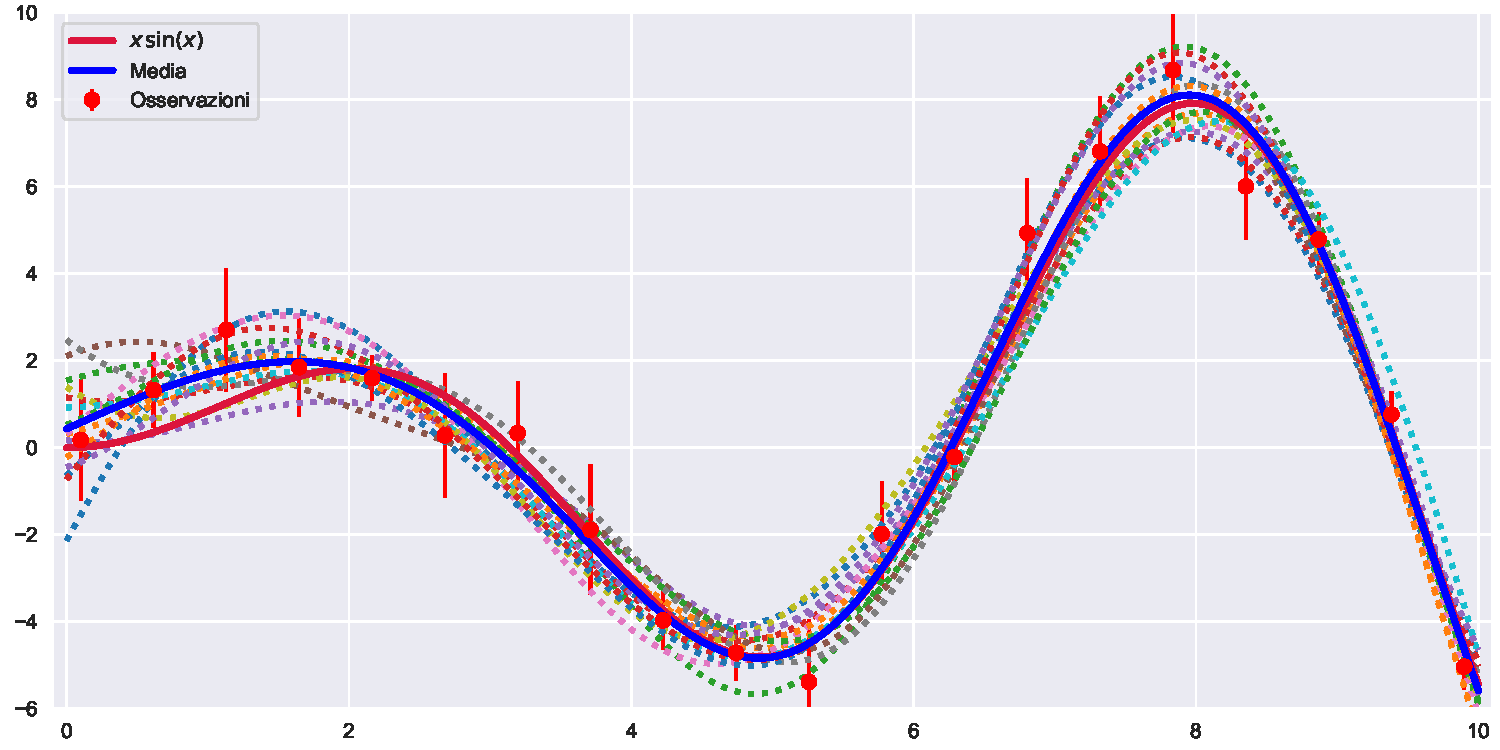
\includegraphics[width=1\textwidth]{images/Gaussian process/Noise - mean&f(x).pdf}
    \caption{Graph of functions with distribution $f\sim \mathcal{GP}(\bm{0},k)$ where $k(\cdot,\cdot)$ is the squared-exponential kernel; the Gaussian process was conditioned to predict a function from its noisy observations. Shown in red is the function to be predicted, in red the observed points of the function with bars representing the noise, in blue the average of the conditioned Gaussian process, as dashed lines some samples of the Gaussian process. Code \ref{Noise code}.}
    \label{Noisy}
\end{figure}

\newpage

Again, the mean of the conditional Gaussian process represents the function that best predicts $x\cdot sin(x)$. Because the observations have error, there is no interpolation of the points although, it tends to be the case that the mean and samples of the Gaussian process touch at least the error bars of each point.
More points of the noise-free case were taken into account since with fewer points such an "accurate" result would not have been obtained (however, with a different behavior from that with noise-free observations).

If in the noiseless case the samples tended to stay near the mean in the vicinity of each interpolated point, here the closeness to the mean depends on both the points and their error: near points with lower noise (i.e., shorter bars) the functions tend to move closer to the mean. Conversely, near features with a large error (longer bars) the features tend to move away from the mean more easily.

Again, the 95\% confidence region can be drawn. The confidence region has amplitude proportional to the length of the bars of the observations; consequently, the confidence region has markedly different behavior from the noise-free case.

%%%%%%%%%%%%%%%%%%%%%%%%%
%%%%%%%%% IMMAGINE
%%%%%%%%%%%%%%%%%%%%%%%%
\begin{figure}[h]
    \centering
    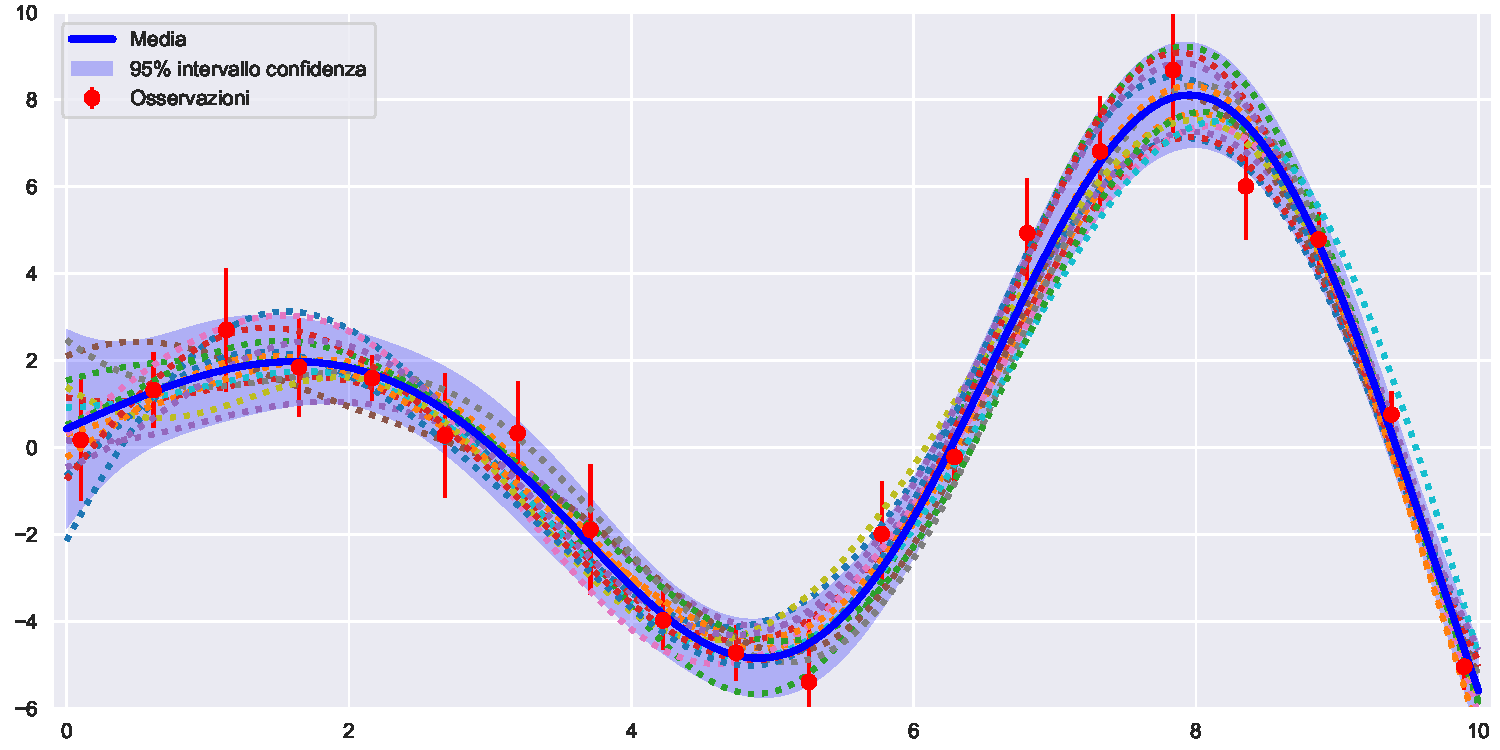
\includegraphics[width=1\textwidth]{images/Gaussian process/Noise - mean&samples.pdf}
    \caption{Graph of functions with distribution $f\sim \mathcal{GP}(\bm{0},k)$ where $k(\cdot,\cdot)$ is the squared-exponential kernel; the Gaussian process was conditioned to predict a function from its noisy observations. Shown in blue is the 95\% confidence region, in red with error bars the observations, in blue the mean of the conditioned Gaussian process, and as dashed lines some samples. Code \ref{Noise confidence region code}.}
    \label{Noisy confidence region}
\end{figure}